\documentclass[12pt,prb,aps]{revtex4-1}
\usepackage{amsmath}           		          	
\usepackage{graphicx,epstopdf}					
\usepackage{amssymb}
\usepackage{fullpage}
\usepackage{color}
\usepackage{esint}
\pdfoutput = 1 
\newcommand {\bxi}{\mbox{\boldmath$\xi$}}
\allowdisplaybreaks

\begin{document}
\title{Calculation of Vertical Stability in an Inverse Aspect-Ratio Expanded Tokamak Plasma Equilibrium}
\author{Richard Fitzpatrick\,\footnote{rfitzp@utexas.edu}}
\affiliation{Institute for Fusion Studies, Department of Physics, University of Texas at Austin, Austin, TX 78712}

\begin{abstract}
The  stability of vertical modes in an up-down symmetric, aspect-ratio expanded, tokamak plasma equilibrium surrounded by
a conformal resistive wall is calculated. The calculation turns out to be significantly different to previous calculations of the stability
of non-axisymmetric ideal modes in an aspect-ratio expanded equilibrium.  In particular, the role of the toroidal angular momentum flux (which is
identically zero for an axisymmetric mode) is instead played by the electromagnetic energy flux. The conservation of electromagnetic energy is used to prove that the perturbed plasma potential energy matrix is Hermitian. 
Positive triangularity is
found to have a stabilizing effect on the vertical mode in vertically elongated plasmas, whereas negative triangularity has a marked destabilizing effect. It is concluded that finite wall thickness should be taken into account when
calculating the maximum controllable plasma elongation of a tokamak plasma. 
\end{abstract}

\maketitle

\section{Introduction}
It is well known that an increase in  the net toroidal plasma current flowing around a tokamak  leads to an enhancement of both the maximum stable $\beta$ value and the energy confinement time.\cite{troyon,goldston}
The conventional method of maximizing the total plasma current, without degrading the  stability of the system to non-axisymmetric magnetohydrodynamical (MHD) modes, is
to modify the plasma's poloidal cross-section such that it is both vertically elongated and triangular.\cite{jet}  Unfortunately, tokamak plasmas possessing strong cross-sectional shaping
are subject to severe axisymmetric instabilities.\cite{v1,v2} Such instabilities involve bulk vertical motion of the plasma on an Alfv\'{e}nic timescale (i.e., $10^{-7}$\,s), which results in the
sudden and violent termination of the  discharge when it comes into contact with the first wall. It is possible to stabilize an axisymmetric mode by placing a perfectly conducting wall
around the plasma. In reality, the mode remains unstable because  the wall inevitably possesses finite electrical conductivity.\cite{rwm}  However, 
growth time of the mode is increased from the Alfv\'{e}n time to the very much longer characteristic L/R time of the wall.\cite{rwm1,rwm1a,rwm2} Usually, the vacuum vessel plays the role of the wall,
and has an L/R time that is  well in excess of  $10^{-3}$\,s. Such a time is much shorter than the length of the plasma 
discharge, but is still long enough to allow active feedback stabilization of the axisymmetric mode with practical power supplies.\cite{rwm3} 

Ref.~\onlinecite{tj} describes the TJ toroidal tearing mode code, which calculates the stability of an inverse aspect-ratio expanded  tokamak plasma equilibrium  to {\em non-axisymmetric}\/ tearing modes via
asymptotic matching techniques. Ref.~\onlinecite{tj1} describes a generalization of the TJ code that permits it to calculate the stability of the plasma to non-axisymmetric
ideal modes in the presence of a perfectly conducting wall surrounding the plasma. The aim of this paper is to describe a further generalization the TJ code that  allows it to calculate
the stability of the plasma to {\em axisymmetric}\/ ideal modes in the presence of a resistive wall that surrounds the plasma. It might be hope that, in order to investigate axisymmetric
modes,  we could simply take the existing
TJ code and set the toroidal mode number, $n$, to zero. Unfortunately, this simple scheme does not work, as evidenced by the large number of terms involving
$n^{-1}$ in the analysis of Ref.~\onlinecite{tj}. Hence, as described in this paper, it is necessary to redo  much of the TJ analysis for the special case $n=0$. 

The simplified approach to calculating the vertical stability of tokamak plasmas described in this paper is somewhat different to that described in Refs.~\onlinecite{f1} and \onlinecite{f2}.
In fact, Refs.~\onlinecite{f1} and \onlinecite{f2} employ  up-down symmetric, analytic Solov'ev plasma equilibria in which the equilibrium  current jumps discontinuously to zero across the
plasma-vacuum interface. Such equilibria can have arbitrary aspect-ratios, and possess the simplifying property that the perturbed plasma currents generated by vertical instabilities are surface currents that
are localized on the interface. On the other hand, this paper employs realistic diffuse plasma equilibria in which the equilibrium current goes smoothly to zero as the plasma-vacuum interface is crossed,
and in which the perturbed plasma currents associated with vertical instabilities are distributed throughout the plasma volume. 
Our main simplifying approximation is to
restrict the inverse aspect-ratio  of the plasma to only take small values. 

This paper is organized as follows. In Sect.~\ref{geq}, we introduce a general axisymmetric plasma equilibrium. 
In Sect.~\ref{opde}, we examine axisymmetric perturbations to this equilibrium. Magnetic perturbations in the vacuum region
surrounding the plasma are discussed in Sect.~\ref{vacuum}. The stability of the equilibrium to ideal axisymmetric modes is
examined in Sect.~\ref{ideal}. The stability of the equilibrium to axisymmetric resistive wall modes is discussed in Sect.~\ref{rwms}. 
The large aspect-ratio approximation is introduced in Sect.~\ref{large}. The results of the calculations performed with the enhanced version of
the TJ code are presented in Ref.~\ref{results}. Finally, the paper is summarized in Sect.~\ref{summary}. 

\section{General Plasma Equilibrium}\label{geq}
All lengths  in this paper  are normalized to  the major radius of the plasma magnetic axis, $R_0$. All magnetic field-strengths
are normalized to the  toroidal field-strength at the magnetic axis, $B_0$. All current densities are normalized to $B_0/(\mu_0\,R_0)$. 
 All plasma pressures are normalized to $B_0^{\,2}/\mu_0$. All energies are normalized to $B_0^{\,2}\,R_0^{\,3}/\mu_0$. 

Let $R$, $\phi$, $Z$ be right-handed cylindrical coordinates whose Jacobian 
is
$(\nabla R\times \nabla\phi\cdot\nabla Z)^{-1} = R$. 
Note that $|\nabla\phi|=1/R$. 
Let $r$, $\theta$, $\phi$ be right-handed flux-coordinates whose
Jacobian is\,\cite{bussac,connor}
\begin{equation}\label{jac}
{\cal J}(r,\theta)\equiv (\nabla r\times \nabla\theta\cdot\nabla\phi)^{-1} \equiv R\left(\frac{\partial R}{\partial\theta}\,\frac{\partial Z}{\partial r} -\frac{\partial R}{\partial r}\,\frac{\partial Z}{\partial \theta}\right)= r\,R^{\,2}.
\end{equation}
Note that $r=r(R,Z)$ and $\theta=\theta(R,Z)$. 
The magnetic axis corresponds to $r=0$. The plasma-vacuum interface corresponds to $r=a$. The inboard mid-plane corresponds to $\theta=0$. 

Consider an axisymmetric tokamak equilibrium whose magnetic field takes the form
\begin{equation}
{\bf B}(r,\theta) = f(r)\,\nabla\phi\times \nabla r + g(r)\,\nabla\phi = f\,\nabla(\phi-q\,\theta)\times \nabla r,
\end{equation}
where
\begin{equation}\label{q}
q(r) = \frac{r\,g}{f}
\end{equation}
is the safety-factor profile. Note that ${\bf B}\cdot\nabla r=0$, which implies that $r$ is a magnetic flux-surface label.
We require $g=1$ on the magnetic axis in order to ensure that the normalized toroidal magnetic field-strength at the  axis is unity.  

It is easily demonstrated that\,\cite{tj}
\begin{align}
B^{\,r}&={\bf B}\cdot\nabla r= 0,\label{bup1}\\[0.5ex]
B^{\,\theta} &={\bf B}\cdot\nabla \theta= \frac{f}{r\,R^{\,2}},\label{bup2}\\[0.5ex]
B^{\,\phi} &={\bf B}\cdot\nabla \phi= \frac{g}{R^{\,2}}= \frac{q\,f}{r\,R^{\,2}},\label{bup3}\\[0.5ex]
B_r &={\cal J}\,\nabla\theta\times\nabla\phi\cdot{\bf B}= -r\,f\,\nabla r\cdot\nabla\theta,\label{bdown1}\\[0.5ex]
B_\theta &={\cal J}\,\nabla\phi\times\nabla r\cdot{\bf B}= r\,f\,|\nabla r|^2,\\[0.5ex]
B_\phi &={\cal J}\,\nabla r\times\nabla \theta \cdot{\bf B}= g.\label{bdown3}
\end{align}

The Maxwell equation (neglecting the displacement current, because the plasma velocity perturbations due to axisymmetric modes are far smaller than the velocity of light in vacuum)
${\bf J}= \nabla\times{\bf B}$
yields
\begin{align}
{\cal J}\,J^{\,r} &= \frac{\partial B_\phi}{\partial \theta} =0,\label{jup1}\\[0.5ex]
{\cal J}\,J^{\,\theta} &= -\frac{\partial B_\phi}{\partial r} = - g',\label{jup2}\\[0.5ex]
{\cal J}\,J^{\,\phi}&= \frac{\partial B_\theta}{\partial r} -\frac{\partial B_r}{\partial\theta}=\frac{\partial}{\partial r}\!\left(r\,f\,|\nabla r|^2\right)+ \frac{\partial}{\partial\theta}\!\left(r\,f\,\nabla r\cdot\nabla\theta\right),\label{jup3}
\end{align}
where ${\bf J}$ is the equilibrium current density, $'\equiv d/dr$, and use has been made of  Eqs.~(\ref{bdown1})--(\ref{bdown3}).

Equilibrium force balance requires that
\begin{equation}\label{e15c}
 \nabla P={\bf J}\times {\bf B},
\end{equation}
where $P(r)$ is the equilibrium scalar plasma pressure. Here, for the sake of simplicity, we have neglected the small centrifugal modifications to force balance due to subsonic plasma
rotation.\cite{flow,flow1}
It follows that 
\begin{align}\label{eg1}
P'&= {\cal J}(J^{\,\theta}\,B^{\,\phi}-J^{\,\phi}\,B^{\,\theta})= -g'\,\frac{g}{R^{\,2}} - \frac{f}{r\,R^{\,2}}\left[\frac{\partial}{\partial r}\!\left(r\,f\,|\nabla r|^2\right)+ \frac{\partial}{\partial\theta}\!\left(r\,f\,\nabla r\cdot\nabla\theta\right)\right],
\end{align}
where use has been made of Eqs.~(\ref{bup1})--(\ref{bup3}), and  (\ref{jup1})--(\ref{jup3}). The
other two components of Eq.~(\ref{e15c}) are identically zero. 

Equation~(\ref{eg1}) yields the {\em inverse Grad-Shafranov equation}:\cite{connor}
\begin{equation}\label{gs}
\frac{f}{r}\,\frac{\partial}{\partial r}\!\left(r\,f\,|\nabla r|^2\right) +\frac{f}{r}\,\frac{\partial}{\partial\theta}\!\left(r\,f\,\nabla r\cdot\nabla\theta\right)+g\,g' + R^{\,2}\,P'=0.
\end{equation}
It follows from Eqs.~(\ref{q}), (\ref{jup3}), and (\ref{gs}) that
\begin{equation}\label{jup3a}
{\cal J}\,J^{\,\phi} = -q\,g' - \frac{r\,R^{\,2}\,P'}{f}.
\end{equation}
It is clear from Eqs.~(\ref{jup2}) and (\ref{jup3a}) that $g'=P'=0$ in the  current-free ``vacuum'' region surrounding the plasma, $r\geq a$. 
We shall also assume that $g'=P'=0$ at the plasma-vacuum interface, so as to ensure that the equilibrium plasma
current density is zero at the interface, $r=a$. 

\section{General Axisymmetric Plasma Perturbation}\label{opde}

\subsection{Derivation of Axisymmetric Ideal-MHD P.D.E.s}\label{pde}
Let us assume that no perturbed quantities depend on  the toroidal angle, $\phi$. 
The perturbed plasma equilibrium satisfies the  linearized, marginally-stable, ideal-MHD equations\,\cite{connor,am1,gs1}
\begin{align}
{\bf b} &= \nabla\times (\bxi\times {\bf B}),\label{e21}\\[0.5ex]
\nabla p &={\bf j}\times {\bf B}  +{\bf J}\times {\bf b},\label{e22}\\[0.5ex]
{\bf j} &= \nabla\times {\bf b},\label{e23}\\[0.5ex]
p&= -\bxi\cdot\nabla P+\delta p,\label{e24}\\[0.5ex]
\delta p &= - {\mit\Gamma}\,P\,\nabla\cdot\bxi,\label{e25ii}
\end{align}
where $\bxi(r,\theta)$ is the plasma displacement, ${\bf b}(r,\theta)$ the perturbed magnetic field,
${\bf j}(r,\theta)$ the perturbed current density, $p(r,\theta)$ the perturbed scalar pressure, and ${\mit\Gamma}=5/3$ the ratio of specific heats.
Here, we are neglecting plasma inertia on the assumption that the wall slows the growth-time of the perturbation such that it is much longer than the Alfv\'{e}n time. 

Now,\cite{tj}
\begin{align}
(\bxi\times {\bf B})_r&= {\cal J}\,(\xi^{\,\theta}\,B^{\,\phi} - \xi^{\,\phi}\,B^{\,\theta}) = f\,(q\,\xi^{\,\theta}-\xi^{\,\phi}),\label{e23xx}\\[0.5ex]
(\bxi\times {\bf B})_\theta&= {\cal J}\,(\xi^{\,\phi}\,B^{\,r} - \xi^{\,r}\,B^{\,\phi}) = -q\,f\,\xi^{\,r},\\[0.5ex]
(\bxi\times {\bf B})_\phi &= {\cal J}\,(\xi^{\,r}\,B^{\,\theta} - \xi^{\,\theta}\,B^{\,r})= f\,\xi^{\,r}\label{e23x}
\end{align}
where use has been made of  Eqs.~(\ref{q}) and (\ref{bup1})--(\ref{bup3}).
 Combining Eqs.~(\ref{e21}) and (\ref{e23xx})--(\ref{e23x}), we obtain\,\cite{tj}
\begin{align}
{\cal J}\,b^{\,r} &= \frac{\partial (\bxi\times {\bf B})_\phi }{\partial\theta}= \frac{\partial (f\,\xi^{\,r})}{\partial\theta},\label{e25tt}\\[0.5ex]
{\cal J}\,b^{\,\theta} &=-\frac{\partial (\bxi\times {\bf B})_\phi }{\partial r}= -\frac{\partial (f\,\xi^{\,r})}{\partial r},\label{e26tt}\\[0.5ex]
{\cal J}\,b^{\,\phi}&=\frac{\partial (\bxi\times {\bf B})_\theta}{\partial r}-\frac{\partial (\bxi\times {\bf B})_r }{\partial \theta}=
 -\frac{\partial (q\,f\,\xi^{\,r})}{\partial r} - \frac{\partial}{\partial\theta}\!\left[f\,(q\,\xi^{\,\theta}-\xi^{\,\phi})\right].\label{e27tt}
\end{align}
Equations~(\ref{jac}), (\ref{e25tt}), and (\ref{e26tt}) give\,\cite{tj}
\begin{align}\label{e41}
r\,R^{\,2}\,b^{\,r}& = \frac{\partial y}{\partial\theta},\\[0.5ex]
r\,R^{\,2}\,b^{\,\theta} &= - \frac{\partial y}{\partial r}.\label{e43y}
\end{align}
where 
\begin{align}\label{e42}
y(r,\theta) &=f\,\xi^{\,r}.
\end{align}
It immediately follows that $\nabla\cdot{\bf b} =0$, in accordance with  Eq.~(\ref{e21}). 
Note that Eq.~(\ref{e43y}) is radically different from the expression, (54), for $b^{\,\theta}$ given in Ref.~\onlinecite{tj}. Thus, it is at this stage that our analysis
starts to diverge from that of Ref.~\onlinecite{tj}.

According to Eq.~(\ref{e24}), 
\begin{equation}
p =-P'\,\nabla r\cdot\bxi+\delta p=- P'\,\xi^{\,r}+ \delta p.
\end{equation}
So, the perturbed force balance equation, (\ref{e22}), yields\,\cite{tj}
\begin{align}
-\frac{\partial\, (P'\,\xi^{\,r})}{\partial r}  +\frac{\partial\,\delta p}{\partial r}&= ({\bf j}\times {\bf B})_r+({\bf J}\times {\bf b})_r,\\[0.5ex]
-\frac{\partial\,(P'\,\xi^{\,r})}{\partial \theta} +\frac{\partial\,\delta p}{\partial \theta}&= ({\bf j}\times {\bf B})_\theta+({\bf J}\times {\bf b})_\theta,\\[0.5ex]
0&= ({\bf j}\times {\bf B})_\phi+({\bf J}\times {\bf b})_\phi,
\end{align}
giving\,\cite{tj}
\begin{align}
-\frac{\partial\, (P'\,\xi^{\,r})}{\partial r}+\frac{\partial\,\delta p}{\partial r} &=r\,R^{\,2}\,(j^{\,\theta}\,B^{\,\phi}-j^{\,\phi}\,B^{\,\theta}) + r\,R^{\,2}\,(J^{\,\theta}\,b^{\,\phi}-J^{\,\phi}\,b^{\,\theta}),\\[0.5ex]
-\frac{\partial\,(P'\,\xi^{\,r})}{\partial \theta} +\frac{\partial\,\delta p}{\partial \theta}&=r\,R^{\,2}\,(j^{\,\phi}\,B^{\,r}-j^{\,r}\,B^{\,\phi}) + r\,R^{\,2}\,(J^{\,\phi}\,b^{\,r}-J^{\,r}\,b^{\,\phi}),\\[0.5ex]
0&=r\,R^{\,2}\,(j^{\,r}\,B^{\,\theta}-j^{\,\theta}\,B^{\,r}) + r\,R^{\,2}\,(J^{\,r}\,b^{\,\theta}-J^{\,\theta}\,b^{\,r}),
\end{align}
where use has been made of Eq.~(\ref{jac}). 
Thus, according to Eqs.~(\ref{bup1})--(\ref{bup3}), (\ref{jup1}), (\ref{jup2}), and (\ref{jup3a}), 
\begin{align}
-\frac{\partial\, (P'\,\xi^{\,r})}{\partial r}  +\frac{\partial\,\delta p}{\partial r}&= f\,(q\,j^{\,\theta} -j^{\,\phi}) - g'\,b^{\,\phi} + \left(q\,g'+\frac{r\,R^{\,2}\,P'}{f}\right)b^{\,\theta},\label{e51}\\[0.5ex]
-\frac{\partial\,(P'\,\xi^{\,r})}{\partial \theta} +\frac{\partial\,\delta p}{\partial \theta}&=-q\,f\,j^{\,r} - \left(q\,g'+\frac{r\,R^{\,2}\,P'}{f}\right)b^{\,r},\label{e44}\\[0.5ex]
0&= f\,j^{\,r}+g'\,b^{\,r}.\label{e53}
\end{align}
It follows from Eqs.~(\ref{e41}) and (\ref{e53}) that 
\begin{equation}\label{e54}
r\,R^{\,2}\,j^{\,r} = -\alpha_g\,\frac{\partial y}{\partial\theta},
\end{equation}
where
\begin{align}
\alpha_g (r)&= \frac{g'}{f}.\label{ag}
\end{align}
Equations~(\ref{e41}), (\ref{e42}), and (\ref{e44}) give 
\begin{equation}\label{e54a}
\delta p = \delta p(r).
\end{equation}
Hence, of the three components of the perturbed force balance equation, only Eq.~(\ref{e51}) remains to be solved. 

Equation~(\ref{e23}) yields\,\cite{tj}
\begin{align}
r\,R^{\,2}\,j^{\,r} &= \frac{\partial b_\phi}{\partial\theta},\label{e57}\\[0.5ex]
r\,R^{\,2}\,j^{\,\theta} &= -\frac{\partial b_\phi}{\partial r},\label{e58}\\[0.5ex]
r\,R^{\,2}\,j^{\,\phi}&= \frac{\partial b_\theta}{\partial r} -\frac{\partial b_r}{\partial \theta},\label{e59}
\end{align}
where use has been made of Eq.~(\ref{jac}). It follows from Eqs.~(\ref{e54}), (\ref{e57}), and (\ref{e58}) that
\begin{align}\label{e43yy}
b_\phi &=-\alpha_g\,y +\delta g(r),\\[0.5ex]
r\,R^{\,2}\,j^{\,\theta}&=  \frac{\partial (\alpha_g\,y-\delta g)}{\partial r}.\label{e44yy}
\end{align}
Note that $\nabla\cdot{\bf j} = 0$, in accordance with Eq.~(\ref{e23}).

Now, 
\begin{equation}
{\bf b} = b_r\,\nabla r + b_\theta\,\nabla\theta+b_\phi\,\nabla\phi,
\end{equation}
so
\begin{align}
b^{\,r} &= {\bf b}\cdot\nabla r = |\nabla r|^2\,b_r + (\nabla r\cdot\nabla\theta)\,b_\theta,\label{e61}\\[0.5ex]
b^{\,\theta} &= {\bf b}\cdot\nabla \theta = (\nabla r\cdot\nabla\theta)\,b_r + |\nabla\theta|^2\,b_\theta,\label{e62}\\[0.5ex]
b^{\,\phi}&={\bf b}\cdot\nabla\phi =\frac{b_\phi}{R^{\,2}}.\label{e63}
\end{align}

Equations~(\ref{jac}), (\ref{e61}), and (\ref{e62}) can be rearranged to give\,\cite{tj}
\begin{align}
b_r &= \left(\frac{1}{|\nabla r|^2}\right)b^{\,r}- \left(\frac{\nabla r\cdot\nabla\theta}{|\nabla r|^2}\right)b_\theta,\label{e69}\\[0.5ex]
\label{e58x}
b^{\,\theta}& = \left(\frac{\nabla r\cdot\nabla\theta}{|\nabla r|^2}\right)b^{\,r} + \left(\frac{1}{r^2\,R^{\,2}\,|\nabla r|^2}\right) b_\theta.
\end{align}
Let 
\begin{equation}\label{zdef}
{\cal Z}(r,\theta)= |\nabla r|^2\,r\,\frac{\partial y}{\partial r} + r\,\nabla r\cdot\nabla\theta\,\frac{\partial y}{\partial\theta}.
\end{equation}
Equations~(\ref{e41}), (\ref{e43y}), (\ref{e43yy}), (\ref{e69}) and (\ref{e58x}) yield 
\begin{align}\label{e53y}
b_r &=\frac{1}{r\,|\nabla r|^2\,R^{\,2}}\,\frac{\partial y}{\partial \theta} + \frac{\nabla r\cdot\nabla\theta}{|\nabla r|^2}\,{\cal Z},\\[0.5ex]
b_\theta &= -{\cal Z},\label{e54y}\\[0.5ex]
b^{\,\phi} &= -\frac{(\alpha_g\,y-\delta g)}{R^{\,2}}.\label{e55yy}
\end{align}
Equations~(\ref{e59}), (\ref{e53y}), and (\ref{e54y}) give
\begin{align}\label{e56yy}
r\,R^{\,2}\,j^{\,\phi} &=-\frac{\partial {\cal Z}}{\partial r}-\frac{\partial}{\partial\theta}\!\left[\frac{1}{r\,|\nabla r|^2\,R^{\,2}}\,\frac{\partial y}{\partial \theta} + \frac{\nabla r\cdot\nabla\theta}{|\nabla r|^2}\,{\cal Z}\right].
\end{align}

It follows from Eqs.~(\ref{e43y}), (\ref{e42}), (\ref{e51}), (\ref{e54a}), (\ref{e44yy}),  (\ref{e55yy}), and (\ref{e56yy}) that
\begin{align}
-\frac{\partial}{\partial r}\!\left(\frac{P'}{f}\,y\right)+\delta p'&= \frac{f\,q}{r\,R^{\,2}}\,\frac{\partial (\alpha_g\,y-\delta g)}{\partial r} 
+ \frac{f}{r\,R^{\,2}}\,\frac{\partial {\cal Z}}{\partial r}\nonumber\\[0.5ex]
&\phantom{=} +\frac{f}{r\,R^{\,2}}\frac{\partial}{\partial\theta}\!\left[\frac{1}{r\,|\nabla r|^2\,R^{\,2}}\,\frac{\partial y}{\partial \theta} + \frac{\nabla r\cdot\nabla\theta}{|\nabla r|^2}\,{\cal Z}\right]
\nonumber\\[0.5ex]
&\phantom{=} + \frac{g'\,(\alpha_g\,y-\delta g)}{R^{\,2}} - \left(q\,g'+\frac{r\,R^{\,2}\,P'}{f}\right)\frac{1}{r\,R^{\,2}}\,\frac{\partial y}{\partial r}.
\end{align}
Hence,
\begin{multline}\label{e58u}
-\left[(\alpha_f\,\alpha_p+ r\,\alpha_p')R^{\,2} + q\,r\,\alpha_g'+r^2\,\alpha_g^2\right]y + \frac{q\,R^{\,2}}{g}\,r\,\delta p' + q\,r\,\delta g' + r^2\,\alpha_g\,\delta g\\[0.5ex]
= r\,\frac{\partial {\cal Z}}{\partial r}+\frac{\partial}{\partial\theta}\!\left[\frac{1}{|\nabla r|^2\,R^{\,2}}\,\frac{\partial y}{\partial \theta} + \frac{r\,\nabla r\cdot\nabla\theta}{|\nabla r|^2}\,{\cal Z}\right],
\end{multline}
and
\begin{equation}\label{jphi}
r^2\,R^{\,2}\,j^{\,\phi} = \left[(\alpha_f\,\alpha_p+ r\,\alpha_p')R^{\,2} + q\,r\,\alpha_g'+r^2\,\alpha_g^2\right]y - \frac{q\,R^{\,2}}{g}\,r\,\delta p' - q\,r\,\delta g' - r^2\,\alpha_g\,\delta g,
\end{equation}
where 
\begin{align}\label{alpp}
\alpha_p(r)&= \frac{r\,P'}{f^2},\\[0.5ex]
\alpha_f(r) &= \frac{r^2}{f}\,\frac{d}{dr}\!\left(\frac{f}{r}\right).\label{alpf}
\end{align}

Equations~(\ref{jac}), (\ref{e27tt}), (\ref{e42}), and (\ref{e55yy}) imply that
\begin{equation}
r\,(\alpha_g\,y-\delta g) = \frac{\partial\,(q\,y)}{\partial r} + \frac{\partial}{\partial\theta}\!\left[f\,(q\,\xi^{\,\theta}-\xi^{\,\phi})\right].
\end{equation}
Hence, we deduce that
\begin{equation}\label{deltag}
r\,\delta g = r\,\alpha_g\,\langle y\rangle - \frac{d\,(q\,\langle y\rangle)}{dr},
\end{equation}
where $\langle \cdots\rangle = \oint(\cdots)\,d\theta/(2\pi)$. Furthermore, Eqs.~(\ref{jac}), (\ref{q}), (\ref{e25ii}), and (\ref{e42})   yield\,\cite{tj}
\begin{equation}
r\,R^{\,2}\,\delta p = - {\mit\Gamma}\,P\left[\frac{\partial}{\partial r}\!\left(\frac{q}{g}\,R^{\,2}\,y\right)+\frac{\partial}{\partial\theta}\!\left(r\,R^{\,2}\,\xi^{\,\theta}\right)\right],
\end{equation}
which gives
\begin{equation}\label{deltap}
r\,\langle R^{\,2}\rangle\,\delta p = -{\mit\Gamma}\,P\,\frac{d}{dr}\!\left(\frac{q}{g}\,\langle R^{\,2}\,y\rangle\right).
\end{equation}

Let us now assume that 
\begin{equation}\label{sym}
\langle y\rangle = \langle R^{\,2}\,y\rangle = 0,
\end{equation}
as would be the case for a purely vertical displacement in an up-down symmetric plasma equilibrium.\cite{f1}
In this case, Eqs.~(\ref{deltag}) and (\ref{deltap}) yield 
\begin{equation}\label{e70tt}
\delta g = \delta p = 0,
\end{equation}
 which, from Eq.~(\ref{e25ii}),  implies that $\nabla\cdot\bxi=0$. In other words, a purely vertical displacement in an up-down
symmetric equilibrium does not compress the plasma. 

It is clear from Eqs.~(\ref{e54}), (\ref{e44yy}), (\ref{jphi}), and (\ref{e70tt}) that $j^{\,r}=j^{\,\theta}=j^{\,\phi}=0$ in the vacuum region, $r\geq a$, which is characterized by $\alpha_g=\alpha_p=0$. On the
other hand, the contravariant components of the perturbed plasma current are  non-zero throughout the plasma. 

Equations~(\ref{zdef}), (\ref{e58u}), and   (\ref{e70tt}) yield the {\em axisymmetric ideal-MHD partial differential equations (p.d.e.s)},
\begin{align}\label{e63y}
r\,\frac{\partial y}{\partial r} &= \frac{{\cal Z}}{|\nabla r|^2} - \frac{r\,\nabla r\cdot\nabla\theta}{|\nabla r|^2}\,\frac{\partial y}{\partial\theta},\\[0.5ex]
r\,\frac{\partial {\cal Z}}{\partial r}&= -\left[(\alpha_f\,\alpha_p+ r\,\alpha_p')R^{\,2} + q\,r\,\alpha_g'+r^2\,\alpha_g^{\,2}\right]y-\frac{\partial}{\partial\theta}\!\left(\frac{1}{|\nabla r|^2\,R^{\,2}}\,\frac{\partial y}{\partial\theta}\right)\nonumber\\[0.5ex]
&\phantom{=} -\frac{\partial}{\partial\theta}\!\left(\frac{r\,\nabla r\cdot\nabla\theta}{|\nabla r|^2}\,{\cal Z}\right),\label{e64y}
\end{align}
which govern the perturbed equilibrium. 

\subsection{Derivation of the Axisymmetric Ideal-MHD O.D.E.s}\label{ode}
Let
\begin{align}\label{e62s}
y(r,\theta)&= \sum_m y_m(r)\,{\rm e}^{\,{\rm i}\,m\,\theta},\\[0.5ex]
{\cal Z}(r,\theta) &= \sum_m Z_m(r)\,{\rm e}^{\,{\rm i}\,m\,\theta}.\label{e63s}
\end{align}
Here, the $m$ are the set of (integer, but not necessarily positive) poloidal mode numbers included in the calculation. 
Equations~(\ref{e63y}) and (\ref{e64y}) yield the {\em axisymmetric ideal-MHD ordinary differential equations (o.d.e.s)}:
\begin{align}\label{e69u}
r\,\frac{dy_m}{dr}&= \sum_{m'}\left(A_{m}^{\,m'}\,Z_{m'} + B_{m}^{\,m'}\,y_{m'}\right),\\[0.5ex]
r\,\frac{dZ_m}{dr}&= \sum_{m'}\left(C_{m}^{\,m'}\,Z_{m'} + D_{m}^{\,m'}\,y_{m'}\right),\label{e70uu}
\end{align}
where
\begin{align}
A_m^{\,m'} &= c_{m}^{\,m'},\\[0.5ex]
B_m^{\,m'} &= - m'\,f_m^{\,m'},\\[0.5ex]
C_{m}^{\,m'} &= -m\,f_m^{\,m'},\\[0.5ex]
D_{m}^{\,m'}&= -(\alpha_f\,\alpha_p+ r\,\alpha_p')\,a_m^{\,m'} - (q\,r\,\alpha_g' +r^{\,2}\,\alpha_g^{\,2})\,\delta_m^{\,m'}+m\,m'\,b_m^{\,m'},\label{Ddef}
\end{align}
and
\begin{align}\label{e73er}
a_m^{\,m'}(r)  &=\oint R^{\,2}\,\exp[-{\rm i}\,(m-m')\,\theta]\,\frac{d\theta}{2\pi},\\[0.5ex]
b_m^{\,m'}(r)  &=\oint|\nabla r|^{-2}\, R^{-2}\,\exp[-{\rm i}\,(m-m')\,\theta]\,\frac{d\theta}{2\pi},\\[0.5ex]
c_m^{\,m'}(r)  &=\oint|\nabla r|^{-2}\,\exp[-{\rm i}\,(m-m')\,\theta]\,\frac{d\theta}{2\pi},\\[0.5ex]
f_{m}^{\,m'}(r)&= \oint \frac{{\rm i}\,r\,\nabla r\cdot\nabla\theta}{|\nabla r|^2}\,\exp[-{\rm i}\,(m-m')\,\theta]\,\frac{d\theta}{2\pi}.\label{e76er}
\end{align}
Here, $\delta_m^{\,m'}$ is a Kronecker delta symbol. Note that $Z_0(r)$ is independent of $r$ in the vacuum region, $r\geq a$,  in which
$\alpha_g=\alpha_p=0$. 

The axisymmetric ideal-MHD o.d.e.s play the same role for axisymmetric perturbations that the outer-region o.d.e.s, (102) and (103) of Ref.~\onlinecite{tj}, play for
non-axisymmetric perturbations. The main difference is that there are no singularities in the axisymmetric ideal-MHD o.d.e.s because an axisymmetric perturbation 
does not resonate with the plasma. In other words, there are no equilibrium flux-surfaces in the plasma at which ${\bf k}\cdot{\bf B}=0$, where ${\bf k}$ is the
wavevector of the perturbation. This is because $|B^{\,\theta}(r)|>0$ throughout a conventional tokamak plasma equilibrium. 

\subsection{Properties of Axisymmetric Ideal-MHD O.D.E.s}
Note   that
$a_{m'}^{\,m} =a_{m}^{\,m'\ast}$, 
$b_{m'}^{\,m} =b_{m}^{\,m'\ast}$, 
$c_{m'}^{\,m} =c_{m}^{\,m'\ast}$, and 
$f_{m'}^{\,m} =-f_{m}^{\,m'\ast}$,
which implies that
\begin{align}\label{e70u}
A_{m'}^{\,m} &= A_{m'}^{\,m\,\ast},\\[0.5ex]
B_{m'}^{\,m} &= -C_{m'}^{\,m\,\ast},\\[0.5ex]
C_{m'}^{\,m} &= -B_{m'}^{\,m\,\ast},\\[0.5ex]
D_{m'}^{\,m} &= D_{m'}^{\,m\,\ast}.\label{e82u}
\end{align}
It follows from Eqs.~(\ref{e69u}), (\ref{e70uu}), and (\ref{e70u})--(\ref{e82u}) that 
\begin{align}\label{cons}
r\,\frac{d}{dr}\!\left[\sum_m (Z_m\,y_m^{\,\ast}- y_m\,Z_m^{\,\ast}) \right]&= 0.
\end{align}

\subsection{Perturbed Electric Field}
Suppose that all perturbed quantities vary in time as ${\rm e}^{-{\rm i}\,\omega\,t}$. 
Let ${\bf e}$ be the perturbed electric field, which satisfies 
\begin{equation}
\nabla\times {\bf e} = {\rm i}\,\omega\,{\bf b}.
\end{equation}
Hence,
\begin{equation}\label{ephi}
e_\phi = {\rm i}\,\omega\,y,
\end{equation}
and 
\begin{equation}\label{e81op}
\frac{\partial e_\theta}{\partial r} - \frac{\partial e_r}{\partial\theta} = - {\rm i}\,\omega\,r\,\alpha_g\,y,
\end{equation}
where use has been made of Eqs.~(\ref{e41}), (\ref{e43y}),  (\ref{e55yy}), and (\ref{e70tt}). 
We also expect $\nabla\cdot{\bf e} =0$, which implies that 
$e_r=e_\theta=0$ in the vacuum region, $r\geq a$, in which $\alpha_g=0$. 

\subsection{Toroidal Electromagnetic Torque}\label{storque}
The net toroidal electromagnetic torque exerted on the region of the plasma lying within the magnetic flux-surface whose label is $r$ is\,\cite{tj}
\begin{equation}
T_\phi(r)= \oint\oint r\,R^{\,2}\,b_\phi\,b^{\,r}\,d\theta\,d\phi.
\end{equation}
It follows from Eqs.~(\ref{e41}) and (\ref{e43yy}) that 
\begin{equation}
T_\phi(r) = -\frac{\pi\,\alpha_g}{2}\oint\left(y^\ast\,\frac{\partial y}{\partial\theta}+y\,\frac{\partial y^\ast}{\partial\theta}\right)d\theta
= -\frac{\pi\,\alpha_g}{2}\oint\frac{\partial|y|^2}{\partial\theta}\,d\theta = 0.
\end{equation}
We conclude, not surprisingly,  that an axisymmetric perturbation is incapable of exerting a net toroidal electromagnetic torque on the plasma. 

In Ref.~\onlinecite{tj1}, the conservation of toroidal angular momentum is used to prove that the plasma and vacuum perturbed potential energy matrices are Hermitian.
The fact that the toroidal electromagnetic torque is identically  zero in the axisymmetric case negates this proof. Hence, we need to find a new conserved quantity
that is not identically zero. The electromagnetic energy flux is found to play this role. 

\subsection{Electromagnetic Energy Flux}
The net flux of electromagnetic energy across the plasma-vacuum interface is 
\begin{align}\label{eflux}
{\cal E}(a) &= \left[\oint\oint ({\bf e}\times {\bf b})\cdot\nabla r\,{\cal J}\,d\theta\,d\phi\right]_{r=a}= \left[\oint\oint (e_\theta\,b_\phi-e_\phi\,b_\theta)\,d\theta\,d\phi\right]_{r=a}\nonumber\\[0.5ex]
&={\rm i}\,\frac{\pi\,\omega}{2}\oint (y\,{\cal Z}^{\,\ast}-y^\ast \,{\cal Z})_{r=a}\,d\theta={\rm i}\,\pi^2\,\omega \sum_{m}\left(Z_m^{\,\ast}\,y_m-y_m^\ast\,Z_m\right)_{r=a}.
\end{align}
Here, use has been made of Eqs.~(\ref{e54y}), (\ref{e62s}), (\ref{e63s}),  and  (\ref{ephi}), as well as  the fact that $e_\theta=0$ for $r\geq a$. 
 Now, Eq.~(\ref{cons}) implies that
$\sum_m(Z_m^{\,\ast}\,y_m-y_m^\ast\,Z_m)$ is independent of $r$. However, we expect $\sum_m(Z_m^{\,\ast}\,y_m-y_m^\ast\,Z_m)=0$ for a well-behaved
solution of the axisymmetric ideal-MHD o.d.e.s close to the magnetic axis ($r=0$). [See Eqs.~(\ref{e234g}) and (\ref{e235g}).] Hence, we deduce that
\begin{equation}\label{excons}
{\cal E}(a) = 0.
\end{equation}
In other words, the net flux of electromagnetic energy out of the plasma is zero. 

\subsection{Perturbed Plasma Potential Energy}
The perturbed plasma potential energy in the region of the plasma lying within the magnetic flux-surface whose label is $r$ is\,\cite{tj1,gs1}
\begin{equation}
\delta W_p(r) = \frac{1}{2}\oint\oint r\,R^{\,2}\,\xi^{\,r\ast}(-{\bf B}\cdot{\bf b} + \xi^{\,r}\,P')\,d\theta\,d\phi.
\end{equation}
Here, we have neglected the contribution to the perturbed energy from plasma compressibility because $\nabla\cdot\bxi= 0$. (See Sect.~\ref{pde}.)
However,
\begin{equation}
{\bf B}\cdot{\bf b} -\xi^{\,r}\,P' = B^{\,\theta}\,b_\theta+B^{\,\phi}\,b_\phi - \xi^{\,r}\,P'
= - \frac{f}{r\,R^{\,2}}\left({\cal Z} + q\,\alpha_g\,y + \alpha_p\,R^{\,2}\right),
\end{equation}
where use has been made of Eqs.~(\ref{q})--(\ref{bup3}), (\ref{e42}), (\ref{e43yy}), (\ref{e54y}),  and (\ref{alpp}). Hence,
we obtain
\begin{align}\label{e87j}
\delta W_p(r) &=\frac{1}{2}\left[\oint\oint y^{\ast}\left({\cal Z} + \alpha_g \,q\,y+ \alpha_p\,R^{\,2}\, y\right)d\theta\,d\varphi\right]_r\nonumber\\[0.5ex]
&=\pi^2\left[\sum_{m}y_m^{\,\ast}\left(Z_m + \alpha_g \,q\,y_m+ \alpha_p\sum_{m'}a_m^{\,m'}\, y_m\right)\right]_r.
\end{align}
 In particular,  the net perturbed plasma potential energy is 
 \begin{equation}\label{e7.34yi}
 \delta W_p(a) =  \pi^2\left(\sum_{m}y_m^{\,\ast}\,Z_m \right)_a,
 \end{equation}
 because $\alpha_g=\alpha_p =0$ at $r=a$. However, it is clear from Equations~(\ref{eflux}) and (\ref{excons}) that $(\sum_m y_m^{\,\ast}\,Z_m)_a$ is real. 
 Hence, we deduce that $\delta W_p(a)$ is real. 

\section{General Vacuum Solution}\label{vacuum}
\subsection{Toroidal Coordinates}
Let $\mu$, $\eta$, $\phi$ be right-handed {\em orthogonal toroidal coordinates}\/ defined such that\,\cite{tj,tj1,mf}
\begin{align}
R &= \frac{\sinh\mu}{\cosh\mu-\cos\eta},\\[0.5ex]
Z&=\frac{\sin\eta}{\cosh\mu-\cos\eta}.
\end{align}
The scale-factors of the toroidal coordinate system are
\begin{align}
h_\mu&=h_\eta= \frac{1}{\cosh\mu-\cos\eta}\equiv h,\\[0.5ex]
h_\phi &= \frac{\sinh\mu}{\cosh\mu-\cos\eta} = h\,\sinh\mu.
\end{align}
Moreover, 
\begin{equation}
{\cal J}' \equiv (\nabla\mu\times\nabla\eta\cdot\nabla\phi)^{-1}= h^3\,\sinh\mu.
\end{equation}

\subsection{Perturbed Magnetic Field}
The curl-free perturbed magnetic field in the vacuum region is written ${\bf b} = {\rm i}\,\nabla V$,
where
$\nabla^2 V =0$.
The most general axisymmetric  solution to Laplace's equation is\,\cite{tj1,mf1}
\begin{align}
V(z,\eta)&= \sum_m (z-\cos\eta)^{1/2}\,U_m(z)\,{\rm e}^{-{\rm i}\,m\,\eta}, \\[0.5ex]
U_m(z) &= p_m\,\hat{P}_{|m|-1/2}(z)+q_m\,\hat{Q}_{|m|-1/2}(z),
\end{align}
where  $z=\cosh\mu$, the $p_m$ and $q_m$ are arbitrary complex coefficients, and 
\begin{align}\label{e21dd}
\hat{P}_{|m|-1/2}(z) &= \cos(|m|\,\pi)\,\frac{\sqrt{\pi}\,\Gamma(|m|+1/2)\,a^{\,|m|}}{2^{\,|m|-1/2}\,|m|!}\,P_{|m|-1/2}(z),\\[0.5ex]
\hat{Q}_{|m|-1/2}(z)&= \cos(|m|\,\pi)\,\frac{2^{\,|m|-1/2}\,|m|!}{\sqrt{\pi}\,\Gamma(|m|+1/2)\,a^{\,|m|}}\,Q_{|m|-1/2}(z).\label{e22dd}
\end{align}
Here,  the $P_{|m|-1/2}(z)$  and $Q_{|m|-1/2}(z)$ are toroidal functions,\cite{as1} and $\Gamma(z)$ is a
gamma function.\cite{as2}

In the large-aspect ratio limit, $r\ll 1$, it can be demonstrated that\,\cite{mf2}
\begin{align}
z&\simeq \frac{1}{r},\label{e25t}\\[0.5ex]
z^{\,1/2}\,\hat{P}_{-1/2}(z) &\simeq \frac{1}{2}\ln\left(\frac{8}{r}\right),\\[0.5ex]
z^{1/2}\,\hat{P}_{|m|-1/2}(z) &\simeq \frac{\cos(|m|\,\pi)\,(r/a)^{-|m|}}{|m|},\label{ety}\\[0.5ex]
z^{1/2}\,\hat{Q}_{|m|-1/2}(z) &\simeq \frac{\cos(|m|\,\pi)\,(r/a)^{|m|}}{2}.\label{e29t}
\end{align}
Note that Eq.~(\ref{ety}) only applies to $|m|>0$.

\subsection{Toroidal Electromagnetic Angular Momentum Flux}
The outward flux of toroidal angular momentum across a constant-$z$ surface is\,\cite{tj,tj1}
\begin{align}
T_\phi(z) &= -\oint\oint {\cal J}' \,b_\phi\,b^{\,\mu}\,d\eta\,d\phi = 0,
\end{align}
because $b_\phi = {\rm i}\,\partial V/\partial\phi = 0$. Of course, the flux has to be zero because the flux of angular momentum across the plasma-vacuum
interface is zero, and there are no sources of angular momentum in the vacuum region surrounding the plasma. (See Sect.~\ref{storque}.)

\subsection{Electromagnetic Energy Flux}
The outward flux of electromagnetic energy flux across a  surface of constant $z$ is
\begin{align}
{\cal E}(z) = -\oint\oint {\cal J}'\,{\bf e}\times {\bf b}\cdot\nabla \mu\,d\eta\,d\phi= -{\rm i}\,
\frac{\pi}{2}\oint\left(e_\phi\,\frac{\partial V^\ast}{\partial\eta}
- e_\phi^{\,\ast}\,\frac{\partial V}{\partial\eta}\right)d\eta,
\end{align}
given that $e_\mu=e_\eta=0$ in the vacuum. 
However, $\nabla\times{\bf e}= {\rm i}\,\omega\,{\bf b}$ implies that
\begin{equation}
\frac{\partial e_\phi}{\partial\eta} = - \omega\,h\,\sinh\mu\,\frac{\partial V}{\partial \mu}= - \omega\,h\,(z^2-1)\,\frac{\partial V}{\partial z}. 
\end{equation}
Thus,
\begin{align}
{\cal E}(z) &= {\rm i}\,\frac{\pi}{2}\oint\left(\frac{\partial e_\phi}{\partial\eta}\,V^\ast - \frac{\partial e_\phi^{\,\ast}}{\partial\eta}\,V\right)d\eta= 
-{\rm i}\,\frac{\pi\,\omega}{2}\oint h\,(z^2-1)\left(\frac{\partial V}{\partial z}\,V^\ast - \frac{\partial V^\ast}{\partial z}\,V\right) d\eta\nonumber\\[0.5ex]
&= {\rm i}\,\pi^2\,\omega\sum_m(p_m\,q_m^{\,\ast}-q_m\,p_m^{\,\ast})\,(z^2-1)\,{\cal W}(P_{|m|-1/2},Q_{|m|-1/2}),
 \end{align}
 where we have integrated by parts, and ${\cal W}(f,g)\equiv f\,dg/dz-g\,df/dz$. However,\cite{mf2}
 \begin{equation}
 {\cal W}(P_{|m|-1/2},Q_{|m|-1/2}) = \frac{1}{1-z^2},
 \end{equation}
 so
 \begin{equation}\label{e168g}
 {\cal E}(z)=- {\rm i}\,\pi^2\,\omega\sum_m(p_m\,q_m^{\,\ast}-q_m\,p_m^{\,\ast}).
 \end{equation}
 Note that ${\cal E}(z)$ is independent of $z$, as must be the case because there are no energy sources in the vacuum region. 

\subsection{Solution in Vacuum Region}
According to Eq.~(\ref{e41}) and (\ref{e54y}),
\begin{align}\label{e30ay}
\frac{\partial y}{\partial \theta}&= {\cal J}\,{\bf b}\cdot\nabla r = {\rm i}\,{\cal J}\,\nabla V\cdot\nabla r,\\[0.5ex]
{\cal Z}&= -{\cal J}\,\nabla\phi\times\nabla r \cdot{\bf b} = - {\rm i}\,\frac{\partial V}{\partial\theta}.\label{e31ay}
\end{align}
Now, we have already seen that $Z_0\equiv \oint{\cal Z}\,d\theta/(2\pi)=0$ is independent of $r$ in the vacuum region.  (See Sect.~\ref{ode}.) 
However, it is clear that Eq.~(\ref{e31ay}) mandates that this constant value is zero. This constraint implies that the axisymmetric ideal modes to
which the plasma equilibrium is subject do not change the net toroidal current flowing in the plasma. [See Eqs.~(\ref{e54y}) and (\ref{ipdef}).]  Note, further, that $y_0\equiv \oint y\,d\theta/(2\pi)$ does
not influence the vacuum potential, $V(r,\theta)$. 

The previous two equations yield\,\cite{tj1}
\begin{align}\label{e32ay}
\underline{V}(r)&= \underline{\underline{{\cal P}}}(r)\,\underline{p}+ \underline{\underline{{\cal Q}}}(r)\,\underline{q},\\[0.5ex]
\underline{\psi}(r)&= \underline{\underline{{\cal R}}}(r)\,\underline{p}+ \underline{\underline{{\cal S}}}(r)\,\underline{q},\label{e33ay}
\end{align}
where $V(r,\theta)= \sum_m V_m(r)\,{\rm e}^{\,{\rm i}\,m\,\theta}$, $Z_m(r)=m\,V_m(r)$, $\psi_m(r)=m\,y_m(r)$, 
 $\underline{V}(r)$ is the vector of the $V_m(r)$ values, $\underline{\psi}(r)$ is the vector of the $\psi_m(r)$ values, $\underline{\underline{{\cal P}}}(r)$ is the
matrix of the
\begin{equation}
{\cal P}_{mm'}(r)=\oint_{r}(z-\cos\eta)^{1/2}\,\hat{P}_{|m'|-1/2}(z)\,\exp[-{\rm i}\,(m\,\theta+m'\,\eta)]\,\frac{d\theta}{2\pi}
\end{equation}
values, 
$\underline{\underline{{\cal Q}}}(r)$ is the
matrix of the
\begin{equation}
{\cal Q}_{mm'}(r)=\oint_{r}(z-\cos\eta)^{1/2}\,\hat{Q}_{|m'|-1/2}(z)\,\exp[-{\rm i}\,(m\,\theta+m'\,\eta)]\,\frac{d\theta}{2\pi}
\end{equation}
values, $\underline{\underline{{\cal R}}}(r)$ is the matrix of the 
\begin{align}\label{e354}
{\cal R}_{mm'}(r) &=\oint_{r}
\left\{\left[\frac{1}{2}\,(z-\cos\eta)^{-1/2}\,\hat{P}_{|m'|-1/2}(z)+(z-\cos\eta)^{1/2}\,\frac{d\hat{P}_{|m'|-1/2}}{dz}\right]{\cal J}\,\nabla r\cdot \nabla z
\right.\nonumber\\[0.5ex]&
\left.\phantom{=}+\left[\frac{1}{2}\,(z-\cos\eta)^{-1/2}\,\sin\eta-{\rm i}\,m'\,(z-\cos\eta)^{1/2}\right]\hat{P}_{|m'|-1/2}(z)\,{\cal J}\,\nabla r\cdot \nabla \eta
\right\}\nonumber\\[0.5ex] &
\phantom{=}\times\exp[-{\rm i}\,(m\,\theta+m'\,\eta)]\,\frac{d\theta}{2\pi}
\end{align}
values, 
$\underline{\underline{{\cal S}}}(r)$ is the matrix of the 
\begin{align}\label{e355}
{\cal S}_{mm'}(r) &=\oint_{r}
\left\{\left[\frac{1}{2}\,(z-\cos\eta)^{-1/2}\,\hat{Q}_{|m'|-1/2}(z)+(z-\cos\eta)^{1/2}\,\frac{d\hat{Q}_{|m'|-1/2}}{dz}\right]{\cal J}\,\nabla r\cdot \nabla z
\right.\nonumber\\[0.5ex]&
\left.\phantom{=}+\left[\frac{1}{2}\,(z-\cos\eta)^{-1/2}\,\sin\eta-{\rm i}\,m'\,(z-\cos\eta)^{1/2}\right]\hat{Q}_{|m'|-1/2}(z)\,{\cal J}\,\nabla r\cdot \nabla \eta
\right\}\nonumber\\[0.5ex] &
\phantom{=}\times\exp[-{\rm i}\,(m\,\theta+m'\,\eta)]\,\frac{d\theta}{2\pi}
\end{align}
values, $\underline{p}$ is the vector of the $p_m$ coefficients, and  $\underline{q}$ is the vector of the $q_m$ coefficients. Here, the
subscript $r$ on the integrals indicates that they are taken at constant $r$. 

\subsection{Energy Conservation}
By analogy with Eq.~(\ref{eflux}), the net flux of electromagnetic energy across a surface of constant $r$ in the vacuum region is
\begin{equation}
{\cal E}(r) = {\rm i}\,\pi^2\,\omega\, (\underline{V}^\dag\,\underline{\psi}- \underline{\psi}^\dag\,\underline{V}).
\end{equation}
However, energy conservation requires this flux to be equal  to the energy flux through the vacuum region, so Eq.~(\ref{e168g}) gives
\begin{equation}\label{e39x}
{\cal E}(r) =-  {\rm i}\,\pi^2\,\omega\,(\underline{q}^\dag\,\underline{p}-\underline{p}^\dag\,\underline{q}).
\end{equation}
Equations~(\ref{e32ay}), (\ref{e33ay}), and the previous two equations, yield\,\cite{tj1}
\begin{align}\label{e41zx}
\underline{\underline{\cal P}}^\dag\,\underline{\underline{\cal R}}&= \underline{\underline{\cal R}}^\dag\,\underline{\underline{\cal P}},\\[0.5ex]
\underline{\underline{\cal Q}}^\dag\,\underline{\underline{\cal S}}&= \underline{\underline{\cal S}}^\dag\,\underline{\underline{\cal Q}},\label{e42zx}\\[0.5ex]
\underline{\underline{\cal P}}^\dag\,\underline{\underline{\cal S}}- \underline{\underline{\cal R}}^\dag\,\underline{\underline{\cal Q}}&=\underline{\underline{1}}.\label{e43zx}
\end{align}
 It can also be demonstrated that 
\begin{align}\label{e46}
\underline{\underline{\cal Q}}\,\underline{\underline{\cal P}}^\dag&= \underline{\underline{\cal P}}\,\underline{\underline{\cal Q}}^\dag,\\[0.5ex]
\underline{\underline{\cal R}}\,\underline{\underline{\cal S}}^\dag&= \underline{\underline{\cal S}}\,\underline{\underline{\cal R}}^\dag.\label{e47x}
\end{align}
The previous five equations hold throughout the vacuum region. 

\subsection{No-Wall Matching Condition}
Suppose that the plasma is surrounded by a vacuum region that extends to infinity. In this case, 
\begin{equation}
\underline{q}=\underline{0},
\end{equation}
 because the 
$\hat{Q}_{|m|-1/2}(z)$ functions blow up in an unphysical manner as $r/a\rightarrow\infty$. [See Eq.~(\ref{e29t})].
It immediately follows from Eq.~(\ref{e39x}) that
 \begin{equation}\label{ezero}
 {\cal E}(z)=0.
 \end{equation}
  In other words, as we would expect, there is zero net flux of electromagnetic energy through the vacuum, because we have already demonstrated that there is zero
  energy flux across the plasma-vacuum interface. [See Equation~(\ref{excons}).]  
Equations~(\ref{e32ay}) and (\ref{e33ay}) imply that
\begin{equation}\label{hdef}
 \underline{V}(r=a_+)= \underline{\underline{H}}\,\underline{\psi}(r=a),
 \end{equation}
 where
 \begin{equation}
 \underline{\underline{H}}= \underline{\underline{\cal P}}_{\,a}\,\underline{\underline{\cal R}}_{\,a}^{-1}
 \end{equation}
 is termed the {\em no-wall vacuum matrix}. 
   Here, $\underline{\underline{\cal P}}_{\,a}= \underline{\underline{\cal P}}(r=a)$, et cetera. 
Equation~(\ref{e41zx}) ensures that  $\underline{\underline{H}}$ is Hermitian. 

\subsection{Perfect-Wall Matching Condition}
Suppose that the plasma is surrounded by a vacuum region that is bounded by a perfectly conducting wall that is conformal to the plasma-vacuum interface, and whose inner surface lies at $r=b_w\,a$, where $b_w\geq 1$. 
Because the wall is perfectly conducting, 
$\underline{\psi}(r=b_w\,a)=\underline{0}$.\cite{gs1}
In other words, the normal component of the perturbed magnetic field is zero at the inner surface of the wall. 
It follows from Eq.~(\ref{e33ay}) that
\begin{equation}
\underline{p} =- \underline{\underline{I}}_b\,\underline{q},
\end{equation}
where
\begin{equation}
 \underline{\underline{I}}_b= \underline{\underline{\cal R}}_{\,b}^{-1}\,\underline{\underline{\cal S}}_{\,b}
 \end{equation}
 is termed the {\em wall matrix}.
 Here, $\underline{\underline{\cal R}}_{\,b}= \underline{\underline{\cal R}}(r=b_w\,a)$, et cetera. Equation~(\ref{e47x}) ensures that $ \underline{\underline{I}}_b$
 is Hermitian. It immediately follows from Eq.~(\ref{e39x}) that
 \begin{equation}\label{ezero1}
 {\cal E}(z)=0.
 \end{equation}
  In other words, as we would again expect, there is zero net flux of electromagnetic energy through the vacuum, because we have already demonstrated that there is zero
  energy flux across the plasma-vacuum interface. [See Equation~(\ref{excons}).]  
 
  Making use of Eqs.~(\ref{e32ay}) and (\ref{e33ay}),  the matching condition at the plasma-vacuum interface  for a perfectly-conducting wall becomes 
 \begin{equation}\label{gdef}
 \underline{V}(r=a_+)= \underline{\underline{G}}\,\underline{\psi}(r=a),
 \end{equation}
 where 
 \begin{equation}
 \underline{\underline{G}}= (\underline{\underline{\cal Q}}_{\,a}-\underline{\underline{\cal P}}_{\,a}\,\underline{\underline{I}}_{\,b})\,(\underline{\underline{\cal S}}_{\,a}-\underline{\underline{\cal R}}_{\,a}\,\underline{\underline{I}}_{\,b})^{-1}
 \end{equation}
 is termed the {\em perfect-wall vacuum matrix}.
It is easily demonstrated from  Eqs.~(\ref{e41zx})--(\ref{e43zx})  that
 \begin{equation}\label{e53xx}
 \underline{\underline{G}}-\underline{\underline{G}}^\dag =- [(\underline{\underline{\cal S}}_{\,a}-\underline{\underline{\cal R}}_{\,a}\,\underline{\underline{I}}_{\,b})^{-1}]^{\dag}\,(\underline{\underline{I}}_{\,b} -\underline{\underline{I}}^\dag_{\,b})\,  (\underline{\underline{\cal S}}_{\,a}-\underline{\underline{\cal R}}_{\,a}\,\underline{\underline{I}}_{\,b})^{-1}.
\end{equation}
Thus,  the perfect-wall vacuum matrix, $\underline{\underline{G}}$, is Hermitian because  the wall matrix, $\underline{\underline{I}}_{\,b}$, is Hermitian. 
 
\subsection{Perturbed Vacuum Potential Energy}
Equation~(\ref{e41}) implies that 
\begin{equation}
{\cal J} \,\nabla r\cdot\nabla V = - {\rm i}\,\frac{\partial y}{\partial \theta}.
\end{equation}
The perturbed potential energy in the vacuum region is\,\cite{tj1,gs1}
\begin{align}
\delta W_v &= \frac{1}{2}\int_{a_+}^\infty \oint\oint {\bf b}^\ast\cdot{\bf b}\,{\cal J}\,dr\,d\theta\,d\phi
=\frac{1}{2}\int_{a_+}^\infty \oint\oint \nabla V^\ast\cdot\nabla V\,{\cal J}\,dr\,d\theta\,d\phi\nonumber\\[0.5ex]
&= -\frac{1}{2}\left(\oint\oint {\cal J}\,\nabla r\cdot\nabla V^\ast\,V\,d\theta\,d\phi\right)_{a_+}
=-\frac{1}{2}\left[\oint\oint \left(-{\rm i}\,\frac{\partial y}{\partial \theta}\right)^\ast\,V\,d\theta\,d\phi\right]_{a_+}\nonumber\\[0.5ex]
&= - \pi^2\left(\sum_m\,m\,y_m^{\,\ast}\,V_m\right)_{a_+},\label{vac}
\end{align}
where use has been made of the facts that $\nabla^2 V =0$, and  $V=0$ at infinity in the no-wall case, and $\nabla r\cdot \nabla V=0$ at the ideal wall in the perfect-wall case. 

\section{General Ideal Stability}\label{ideal}

\subsection{Perturbed Plasma Potential Energy Matrix}\label{ideal1}
Suppose that the poloidal harmonics included in the calculation range from $m=-m_{\rm max}$ to $m=m_{\rm max}$, where $m_{\rm max} >0$. 
Let  the $y_{mm'}(r)$ and the $Z_{mm'}(r)$ be linearly independent solutions of the axisymmetric ideal-MHD o.d.e.s, (\ref{e69u}) and
(\ref{e70uu}), that are well-behaved at the magnetic axis. Here, $m$ indexes the poloidal harmonic, whereas $m'$ indexes the dominant poloidal harmonic close to the magnetic
axis. (See Sect.~\ref{axis}.)
We can form $J=2\,m_{\rm max}$ linearly independent solutions that all have $Z_0=0$ at $r=a$, as mandated by the matching condition (\ref{e31ay}). Let these
new solutions be denoted the $\hat{y}_{mj}(r)$ and the $Z_{mj}(r)$, where $j$ runs from 1 to $J$. 
The most general solution to the axisymmetric ideal-MHD o.d.e.s that satisfies the constraint $Z_0(a)=0$ is written
\begin{align}
y_m(r) &= \sum_{j=1,J} \hat{y}_{mj}(r)\,\alpha_{j'},\\[0.5ex]
Z_m(r)&= \sum_{j=1,J} \hat{Z}_{mj}(r)\,\alpha_{j'},
\end{align}
where the $\alpha_j$ are arbitrary complex coefficients. Here, $m$ indexes the poloidal harmonic and $j$ indexes the solution. 
 
According to Eq.~(\ref{e87j}), the net perturbed plasma potential energy is
\begin{equation}
\delta W_p(a) = \pi^2\,\underline{y}^{\dag}\,\underline{Z},
\end{equation}
where $\underline{y}$ is the vector of the $y_m(a)$ values, excluding the $m=0$ harmonic,  and $\underline{Z}$  the vector of the $Z_m(a_-)$ values,
excluding the $m=0$ harmonic.  We can exclude the $m=0$ harmonic because, by construction, our solutions are such that $Z_0(a_-)=0$. It follows that
\begin{equation}
\delta W_p(a) = \pi^2\,\underline{\alpha}^\dag \,\underline{\underline{y}}^\dag \,\underline{\underline{Z}}\,\underline{\alpha},
\end{equation}
where $\underline{\alpha}$ is the vector of the $\alpha_j$ values, $\underline{\underline{y}}$ the matrix of the $\hat{y}_{mj}(a)$ values, excluding the $m=0$ harmonic, 
and $\underline{\underline{Z}}$ the matrix of the $\hat{Z}_{mj}(a_-)$ values, excluding the $m=0$ harmonic. 
If
\begin{equation}
\underline{\underline{\chi}} = \underline{\underline{W}}_{\,p}\,\underline{\underline{y}}.
\end{equation}
then 
\begin{equation}
\delta W_p(a) = \pi^2\,\underline{\alpha}^\dag \,\underline{\underline{y}}^\dag \,\underline{\underline{W}}_{\,p}\,\underline{\underline{y}}\,\underline{\alpha}.
\end{equation}
We have already shown that $\delta W(a)$ is real, which implies that $\underline{\underline{W}}_{\,p}$, which is known as the {\em perturbed plasma potential energy matrix},
is Hermitian. 

\subsection{Perturbed Vacuum Potential Energy Matrix}
According to Eq.~(\ref{vac}), the perturbed vacuum potential energy is
\begin{equation}
\delta W_v = - \pi^2\sum_m m\,y_m^{\,\ast}(a)\,V_m(a_+),
\end{equation}
excluding the $m=0$ harmonic, which 
obviously does not affect the vacuum energy. 
However, Eqs.~(\ref{hdef}) and (\ref{gdef}) imply that
\begin{equation}
V_m(a_+) = \sum_{m'}\,H_{mm'}\,m'\,y_{m'}(a)
\end{equation}
in the no-wall case, and 
\begin{equation}
V_m(a_+) = \sum_{m'}\,G_{mm'}\,m'\,y_{m'}(a)
\end{equation}
in the perfect-wall case. Here, we have excluded the $m'=0$ harmonic, which also obviously does not affect the vacuum energy. 
Hence, we can write
\begin{equation}
\delta W_v = \pi^2\,\underline{y}^\dag\,\underline{\underline{W}}_{\,v}\,\underline{y},
\end{equation}
where $\underline{\underline{W}}_{\,v}$ is the matrix of the $-m\,H_{mm'}\,m'$ values in the no-wall case, excluding the $m=0$ and $m'=0$ harmonics, and the
$-m\,G_{mm'}\,m'$ values in the perfect-wall case, likewise  excluding the $m=0$ and $m'=0$ harmonics,. Given that $H_{mm'}$ and $G_{mm'}$ are Hermitian, we deduce that $\underline{\underline{W}}_{\,v}$, which is known as the {\em perturbed vacuum potential energy matrix}, 
is Hermitian. It follows that
\begin{equation}
\delta W_v = \pi^2\,\underline{\alpha}^\dag\,\underline{\underline{y}}^\dag\,\underline{\underline{W}}_{\,v}\,\underline{\underline{y}}\,\underline{\alpha}.
\end{equation}

\subsection{Total Perturbed Potential Energy Matrix}
The total perturbed potential energy is
\begin{equation}
\delta W = \delta W_p(a) + \delta W_v = \pi^2\,\underline{\alpha}^\dag\,\underline{\underline{y}}^\dag\,\underline{\underline{W}}\,\underline{\underline{y}}\,\underline{\alpha},
\end{equation}
where 
\begin{equation}
\underline{\underline{W}} = \underline{\underline{W}}_{\,p} + \underline{\underline{W}}_{\,v}.
\end{equation}
Given that $\underline{\underline{W}}_{\,p}$ and $\underline{\underline{W}}_{\,v}$ are both Hermitian, we deduce that $\underline{\underline{W}}$,
which is known as the {\em total perturbed potential energy matrix},  is Hermitian.

\subsection{Ideal Stability}
The fact that $\underline{\underline{W}}$ is Hermitian allows us to write
\begin{align}
\underline{\underline{W}}\,\underline{\underline{\beta}} &= \underline{\underline{\beta}}\,\underline{\underline{\mit\Lambda}},\\[0.5ex]
\underline{\underline{\beta}}^\dag\,\underline{\underline{\beta}} &= \underline{\underline{1}},
\end{align}
where $\underline{\underline{\beta}}$ is real, and $\underline{\underline{\mit\Lambda}}$ is the diagonal matrix of the real $\lambda_m$ values. 
If $\underline{\hat{\alpha}}= \underline{\underline{\beta}}^\dag\,\underline{\underline{y}}\,\underline{\alpha}$ then
\begin{equation}
\delta W =\pi^2\,\underline{\hat{\alpha}}^\dag\,\underline{\underline{\mit\Lambda}}\,\underline{\hat{\alpha}}=\pi^2\sum_{m=1,J}|\hat{\alpha}_m|^2\,\lambda_m.
\end{equation}
Thus, if any of the $\lambda_m$ are negative then solutions exist for which $\delta W$ is negative, and the plasma is consequently unstable to
an axisymmetric ideal mode.\cite{gs1}

Suppose that $\sum_{m}|\hat{\alpha}_m|^2=1$. The ideal energy of the $m$th mode,
for which $\hat{\alpha}_{m'} = \delta_{mm'}$,  is
\begin{equation}
\delta W_m = \pi^2\,\lambda_m.
\end{equation}
However,
\begin{equation}
\underline{\underline{\mit\Lambda}} = \underline{\underline{\beta}}^\dag\,\underline{\underline{W}}\,\underline{\underline{\beta}},
\end{equation}
Thus, the diagonal components of $\underline{\underline{\beta}}^\dag\,\underline{\underline{W}}_{\,p}\,\underline{\underline{\beta}}$ 
and $\underline{\underline{\beta}}^\dag\,\underline{\underline{W}}_{\,v}\,\underline{\underline{\beta}}$  are the plasma and vacuum
contributions to the $\lambda_m$, respectively. 
 The eigenfunction of the $m$th mode is conveniently normalized such that $y_{m'}(a)= \beta_{m'm}$. 
 
\section{General Resistive Wall Mode Stability}\label{rwms}
The unnormalized minor radius of the wall is $b=b_w\,\bar{a}$, where $\bar{a}=\epsilon\,R_0$  is the unnormalized minor radius of the plasma. Suppose that the wall is resistive, and possesses an (unnormalized)  electrical conductivity $\sigma_w$, as well as an (unnormalized)  uniform radial thickness $d$. 
Consider a particular axisymmetric ideal mode for which the total perturbed potential energy in the absence of a wall, 
 $\delta W_{nw}$, is negative,  but the total perturbed potential energy in the presence of a perfectly conducting wall, $\delta W_{pw}$, is positive.  In this case,  the no-wall ideal mode is unstable (because $\delta W_{nw}<0$). In the absence of  the wall, this mode would grow very rapidly on an Alfv\'{e}nic timescale. On the other
 hand, the mode is completely stabilized if the wall is perfectly conducting (because $\delta W_{pw}>0$).  However, because the wall is not perfectly conducting, the unstable ideal mode is
 instead converted into a much more slowly growing {\em resistive wall mode}. 
 
 Let the (unnormalized) 
 growth-rate of the resistive wall mode be
 \begin{equation}
 \gamma= \frac{\hat{\gamma}}{\tau_w},
 \end{equation}
 where
 \begin{equation}
 \tau_w = \mu_0\,\sigma_w\,b\,d
 \end{equation}
 is the (unnormalized) L/R time of the wall. 
 The normalized growth-rate of the resistive wall mode is specified by\,\cite{rwm4,rwm5}
 \begin{equation}\label{rwm}
 \sqrt{\frac{\hat{\gamma}}{\delta_w}}\tanh\left(\sqrt{\delta_w\,\hat{\gamma}}\right) = -\frac{\delta W_{nw}}{\alpha_w\,\delta W_{pw}},
 \end{equation}
 where $\delta_w=d/b$, 
and
 \begin{equation}
 \alpha_w = \frac{(1/2)\int|{\bf A}_{nw}\times {\bf n}_w|^2\,dS_w}{\epsilon\,b_w\,(\delta W_{v\,pw}- \delta W_{v\,nw})}.
 \end{equation}
 Here, $\delta W_{v\,nw}$ is the vacuum potential energy in the absence of a wall, whereas $\delta W_{n\,pw}$ is the vacuum energy in the presence of a
 perfectly conducting wall. 
 Moreover, $dS_w$ is an element of the inner  surface of the wall, and the integral is over the whole inner surface. Furthermore,
 the perturbed magnetic field in the vacuum region, in the no-wall case, is written $\nabla\times {\bf A}_{nw}$. 
 It is easily demonstrated from Eqs.~(\ref{e41}) and (\ref{e43y}) that ${\bf A}_{nw}= \sum_{m} y_{m\,nw}(r)\,{\rm e}^{\,{\rm i}\,m\,\theta}\,\nabla\phi$,
 where the $y_{m\,nw}(r)$ are the $y$-components of the no-wall eigenfunction of the mode in question. Here, we have made use of the fact that $b^{\,\phi}=0$
 in the vacuum region, because $\alpha_g=0$. [See Eqs.~(\ref{e55yy}) and (\ref{e70tt}).]
  Finally, $dS_w= {\cal J}\,d\theta\,d\phi$. 
 Hence, we deduce that
 \begin{equation}\label{alphaw}
 \alpha_w = \frac{\pi^2\left(\sum_{m\neq 0} |y_{m\,nw}|^2\right)_{\hat{r}=b_w}}{\delta W_{v\,pw}- \delta W_{v\,nw}}.
 \end{equation}
 Here, we have neglected $y_{0\,nw}$ because $y_0$ does not affect the vacuum energy. (See Sect.~\ref{ideal1}.)
 
 Given that $\underline{q}=\underline{0}$ for a no-wall solution, Eq.~(\ref{e33ay}) yields  
 \begin{equation}
\underline{\underline{m}}\, \underline{y}_b = \underline{\underline{\cal R}}_{\,b}\,\underline{\underline{\cal R}}_{\,a}^{-1}\,\underline{\underline{m}}\,\underline{y}_a,
\end{equation}
which enables us to determine the $y_{m\neq 0\,nw}(\hat{r}=b_w)$ from the $y_{m\neq 0\,nw}(\hat{r}=1)$. Here, $\underline{\underline{m}}$ is the diagonal matrix of the poloidal
mode numbers. 

Finally, in the {\em thin-wall}\/ limit, $\delta_w\ll 1$, Eq.~(\ref{rwm}) simplifies to give 
 \begin{equation}\label{rwm1}
 \hat{\gamma}= -\frac{\delta W_{nw}}{\alpha_w\,\delta W_{pw}}.
 \end{equation}

\section{Inverse Aspect-Ratio Expanded Tokamak Equilibrium}\label{large}

\subsection{Introduction}
Up to now, our analysis has been completely general. At this stage, we introduce the simplifying approximation of an  inverse aspect-ratio expanded plasma equilibrium. 
However, as discussed in Sect.~\ref{pde}, we must restrict our discussion to up-down symmetric equilibria in order to ensure that $\nabla\cdot\bxi=0$. 

\subsection{Equilibrium Magnetic Flux-Surfaces}\label{flux}
Let us assume that the inverse aspect-ratio of the plasma, $\epsilon=a/R_0=a$ (since $R_0$ is normalized to unity), is such that $0<\epsilon\ll 1$.  
Let $r=\epsilon\,\hat{r}$, $\nabla =\epsilon^{\,-1}\,\hat{\nabla}$, and $'\rightarrow \epsilon^{\,-1}\,'$. 
Suppose that the loci of the up-down symmetric equilibrium magnetic flux-surfaces can be written in the parametric form:\,\cite{tj,tj1,connor}
\begin{align}
R(\hat{r},\omega) &= 1 -\epsilon\,\hat{r}\,\cos\omega + \epsilon^{\,2}\,\sum_{j>0}H_j(\hat{r})\,\cos[(j-1)\,\omega] +\epsilon^{\,3}\,L(\hat{r})\,\cos\omega,\label{e19x}\\[0.5ex]
Z(\hat{r},\omega)&= \epsilon\,\hat{r}\,\sin\omega +\epsilon^{\,2}\,\sum_{j>1}H_j(\hat{r})\,\sin[(j-1)\,\omega]-\epsilon^{\,3}\,L(\hat{r})\,\sin\omega,\label{e20x}
\end{align}
where $j$ is a positive integer. 
Here, $H_1(\hat{r})$  controls the relative horizontal locations of the flux-surface centroids, $H_2(\hat{r})$ controls the 
the flux-surface elongation, $H_3(\hat{r})$  controls the flux-surface triangularity, et cetera, whereas $L(\hat{r})$ is a
flux-surface re-labelling parameter. Moreover, $\omega(R,Z)$ is a  poloidal angle that is distinct from $\theta$. 

Let
\begin{equation}
J(\hat{r},\omega) = \frac{1}{\epsilon^{\,2}}\left(\frac{\partial R}{\partial\omega}\,\frac{\partial Z}{\partial \hat{r}} -\frac{\partial R}{\partial \hat{r}}\,\frac{\partial Z}{\partial \omega}\right)
\end{equation}
be the Jacobian of the $\hat{r}$, $\omega$ coordinate system. We can transform to the $\hat{r}$, $\theta$ coordinate system 
by writing
\begin{align}\label{e11}
\theta(\hat{r},\omega) &= \left.2\pi\int_0^\omega \frac{J(\hat{r},\tilde{\omega})}{R(\hat{r},\tilde{\omega})}\,d\tilde{\omega}\right/\oint\frac{J(\hat{r},\omega)}{R(\hat{r},\omega)}\,d\omega,\\[0.5ex]
\hat{r}&=\frac{1}{2\pi}\oint\frac{J(\hat{r},\omega)}{R(\hat{r},\omega)}\,d\omega.\label{e12}
\end{align}
This transformation ensures that 
\begin{equation}
\frac{\partial\theta}{\partial\omega} = \frac{J}{\hat{r}\,R},
\end{equation}
and, hence, that 
\begin{equation}
{\cal J} \equiv \frac{R}{\epsilon} \left(\frac{\partial R}{\partial\theta}\,\frac{\partial Z}{\partial \hat{r}} -\frac{\partial R}{\partial \hat{r}}\,\frac{\partial Z}{\partial \hat{r}}\right)
=\epsilon\, R\,J\,\frac{\partial\omega}{\partial\theta} =r\,R^{\,2},
\end{equation}
in accordance with Eq.~(\ref{jac}). 

\subsection{Metric Elements}\label{metric}
We can determine the metric elements of the flux-coordinate system by combining Eqs.~(\ref{e19x})--(\ref{e12}).
Evaluating the elements up to ${\cal O}(\epsilon)$, but retaining ${\cal O}(\epsilon^{\,2})$ contributions to terms that are independent of
$\omega$, we obtain,\cite{tj,tj1}
\begin{align}\label{epdef}
L(\hat{r})&= \frac{\hat{r}^{\,3}}{8} -\frac{\hat{r}\,H_1}{2}-\frac{1}{2}\sum_{j>1}(j-1)\,\frac{H_j^{\,2}}{\hat{r}},\\[0.5ex]
\theta &= \omega+\epsilon\,\hat{r}\,\sin\omega - \epsilon\sum_{j>0}\frac{1}{j}\left[H_j'-(j-1)\,\frac{H_j}{\hat{r}}\right]\sin(j\,\omega),\label{e22y}\\[0.5ex]
|\hat{\nabla} \hat{r}|^2 &= 1 +2\,\epsilon\sum_{j>0}H_j'\,\cos(j\,\theta)  \nonumber\\[0.5ex]
&\phantom{=}+\epsilon^{\,2}\left(\frac{3\,\hat{r}^{\,2}}{4}-H_1+
\frac{1}{2}\sum_{j>0}\left[H_j'^{\,2}+(j^2-1)\,\frac{H_j^{\,2}}{\hat{r}^{\,2}}\right]\right),\label{e19}\\[0.5ex]
\hat{\nabla}\hat{r}\cdot\hat{\nabla}\theta&=\epsilon\,\sin\theta
-\epsilon\sum_{j>0}\frac{1}{j}\left[H_j''+\frac{H_j'}{\hat{r}}+(j^2-1)\,\frac{H_j}{\hat{r}^{\,2}}\right]\sin(j\,\theta),\label{e20uu}
\\[0.5ex]
R^{\,2}&= 1-2\,\epsilon\,\hat{r}\,\cos\theta -\epsilon^{\,2}\left(\frac{\hat{r}^{\,2}}{2}-\hat{r}\,H_1'-2\,H_1\right).\label{e25a}
\end{align}
Here, $'\equiv d/d\hat{r}$.

\subsection{Expansion of Inverse Grad-Shafranov Equation}\label{exp}
Let us write\,\cite{tj,tj1}
\begin{align}\label{e26v}
f(\hat{r})&= \epsilon\,\frac{\hat{r}\,g}{q},\\[0.5ex]
g(\hat{r}) &= 1+ \epsilon^{\,2}\,g_2(\hat{r}) + \epsilon^{\,4}\,g_4(\hat{r}),\label{e27v}\\[0.5ex]
P'(\hat{r}) &= \epsilon^{\,2}\,p_2'(\hat{r}),\label{eq1}
\end{align}
where $q$,  $g_2$, $g_4$, and $p_2$ are all ${\cal O}(1)$. Here, the safety-factor, $q(\hat{r})$, and the second-order plasma
pressure gradient, $p_2'(\hat{r})$, are the two free flux-surface functions that characterize the plasma equilibrium.

Expanding the inverse Grad-Shafranov equation, (\ref{gs}), order by order in the
small parameter $\epsilon$, making use of Eqs.~(\ref{e19})--(\ref{eq1}), we obtain\,\cite{am1,tj,tj1}
\begin{align}
g_2'&=- p_2' - \frac{\hat{r}}{q^2}\,(2-s),\label{e26}\\[0.5ex]
H_1''&= -(3-2\,s)\,\frac{H_1' }{\hat{r}}
-1+\frac{2\,p_2'\,q^2}{\hat{r}},\label{e27}\\[0.5ex]
H_j''&= -(3-2\,s)\,\frac{H_j'}{\hat{r}}+(j^2-1)\,\frac{H_j}{\hat{r}^{\,2}}~~~~~\mbox{for $j>1$},\label{e33x}\\[0.5ex]
g_4'&= g_2\left[p_2' - \frac{\hat{r}}{q^2}\,(2-s)\right] - \frac{\hat{r}}{q}\,{\mit\Sigma}
+p_2'\left(\frac{\hat{r}^{\,2}}{2}+\frac{\hat{r}^{\,2}}{q^2}-2\,H_1-3\,\hat{r}\,H_1'\right),\label{e31}
\end{align}
where $s=\hat{r}\,q'/q$ is the magnetic shear, and  
\begin{align}{\mit\Sigma} &=\frac{S_2}{q}- \frac{2-s}{q}\,S_3,\\[0.5ex]
S_1(\hat{r})&=\frac{1}{2}\sum_{j>0} \left[3\,H_j'^{\,2} -(j^2-1)\,\frac{H_j^{\,2}}{\hat{r}^2}\right],\label{e109}
\\[0.5ex]
S_2(\hat{r})&=\frac{3\,\hat{r}^{\,2}}{2} -2\,\hat{r}\,H_1'+\sum_{j>0}\left[H_j'^{\,2}+2\,(j^2-1)\,\frac{H_j'\,H_j}{\hat{r}}-(j^2-1)\,\frac{H_j^{\,2}}{\hat{r}^{\,2}}\right],\\[0.5ex]
S_3(\hat{r})&=-\,\frac{3\,\hat{r}^{\,2}}{4}+\frac{\hat{r}^{\,2}}{q^2} +H_1+S_1,\\[0.5ex]
S_4(\hat{r}) &= \frac{7\,\hat{r}^{\,2}}{4}-H_1 -3\,\hat{r}\,H_1' + S_1.
\end{align}
Note that the relative horizontal shift of magnetic flux-surfaces, $-H_1$, otherwise known as the {\em Shafranov shift}, is driven by toroidicity [the second term on
the right-hand side of Eq.~(\ref{e27})], and plasma pressure gradients (the third term). All of the other shaping terms (i.e., the $H_j$ for $j>1$) are driven by axisymmetric currents flowing in external  magnetic field-coils.

Equations~(\ref{ag}), (\ref{alpp}), (\ref{alpf}), and (\ref{e26v})--(\ref{eq1}) yield\,\cite{tj}
\begin{align}
\alpha_p(\hat{r}) &= \frac{p_2'\,q^2}{\hat{r}}\left(1-2\,\epsilon^{\,2}\,g_2\right),\\[0.5ex]
\alpha_g(\hat{r}) &= \frac{q}{\hat{r}}\left(g_2' -\epsilon^{\,2}\,g_2\,g_2'+\epsilon^{\,2}\,g_4'\right),\\[0.5ex]
\alpha_f(\hat{r}) &= -s + \epsilon^{\,2}\,\hat{r}\,g_2'.
\end{align}
Finally, it follows from Eqs.~(\ref{e20uu}) and (\ref{e27})--(\ref{e33x}) that
\begin{align}\label{e114}
\hat{\nabla}\hat{r}\cdot\hat{\nabla}\theta &= 2\,\epsilon\left[1-\frac{p_2'\,q^2}{\hat{r}} +(1-s)\,\frac{H_1'}{\hat{r}}\right]\sin\theta\nonumber\\[0.5ex]
&\phantom{=}-2\,\epsilon\sum_{j>1}\frac{1}{j}\left[-(1-s)\,\frac{H_j'}{\hat{r}} + (j^2-1)\,\frac{H_j}{\hat{r}^{\,2}}\right]\sin(j\,\theta).
\end{align}

\subsection{Calculation of Coupling Coefficients}
Equations~(\ref{e19}) and (\ref{e109}) yield 
\begin{align}\label{e115}
|\hat{\nabla}\hat{r}|^{-2} &= 1 - 2\,\epsilon\sum_{j>0}H_j'\,\cos(j\,\theta)  
+ \epsilon^2\left(-\frac{3\,\hat{r}^{\,2}}{4} + H_1 + S_1\right),
\end{align}
Equation~(\ref{e25a}) gives
\begin{align}
R^{-2}= 1 + 2\,\epsilon\,\hat{r}\,\cos\theta +\epsilon^2\left(\frac{5\,\hat{r}^{\,2}}{2} - \hat{r}\,H_1'-2\,H_1\right).
\end{align}
The previous two equations imply that
\begin{align}\label{e117}
|\hat{\nabla}\hat{r}|^{-2} \,R^{-2}&= 1 +2\,\epsilon\,\hat{r}\,\cos\theta -2\,\epsilon \sum_{j>0}H_j'\,\cos(j\,\theta) + \epsilon^2\left(\frac{7\,\hat{r}^{\,2}}{4} - H_1 -3\,\hat{r}\,H_1' + S_1\right).
\end{align}
Finally, Eqs.~(\ref{e114}) and (\ref{e115}) yield
\begin{align}\label{e118}
\hat{\nabla}\hat{r}\cdot\hat{\nabla}\theta \,|\hat{\nabla}\hat{r}|^{-2} &= 2\,\epsilon\left[1-\frac{p_2'\,q^2}{\hat{r}} +(1-s)\,\frac{H_1'}{\hat{r}}\right]\sin\theta\nonumber\\[0.5ex]
&\phantom{=}-2\,\epsilon\sum_{j>1}\frac{1}{j}\left[-(1-s)\,\frac{H_j'}{\hat{r}} + (j^2-1)\,\frac{H_j}{\hat{r}^{\,2}}\right]\sin(j\,\theta).
\end{align}

Equations~(\ref{e73er})--(\ref{e76er}), (\ref{e25a}), (\ref{e115}), (\ref{e117}), and (\ref{e118}) imply that
\begin{align}\label{e120}
a_m^{\,m'} &= \delta_{m}^{\,m'} -\epsilon\,\hat{r}\left(\delta_{m'-m-1}+\delta_{m'-m+1}\right)-\epsilon^2\left(\frac{\hat{r}^{\,2}}{2}-\hat{r}\,H_1'-2\,H_1\right)\delta_m^{\,m'},\\[0.5ex]
b_m^{\,m'}&= \delta_m^{\,m'}+\epsilon\,\hat{r}\left(\delta_{m'-m-1}+\delta_{m'-m+1}\right)-\epsilon\sum_{j>0}H_j'\left(\delta_{m'-m-j}+\delta_{m'-m+j}\right)\nonumber\\[0.5ex]
&+ \epsilon^2\left(\frac{7\,\hat{r}^{\,2}}{4} - H_1 -3\,\hat{r}\,H_1' + S_1\right)\delta_{m}^{\,m'},\\[0.5ex]
c_m^{\,m'} &= \delta_m^{\,m'}-\epsilon\sum_{j>0}H_j'\left(\delta_{m'-m-j}+\delta_{m'-m+j}\right)+ \epsilon^2\left(-\frac{3\,\hat{r}^{\,2}}{4} + H_1 + S_1\right)\delta_{m}^{\,m'},\\[0.5ex]
f_m^{\,m'} &= -\epsilon\left[\hat{r} - p_2'\,q^2+ (1-s)\,H_1'\right]\left(\delta_{m'-m-1}-\delta_{m'-m+1}\right) \nonumber\\[0.5ex]
&\phantom{=}+ \epsilon\sum_{j>1}\frac{1}{j}\left[-(1-s)\,H_j'+(j^2-1)\,\frac{H_j}{\hat{r}}\right]\left(\delta_{m'-m-j}-\delta_{m'-m+j}\right).\label{e123}
\end{align}

If we write
\begin{align}
\alpha_g&= \alpha_g^{\,(0)} + \epsilon^2\,\alpha_g^{\,(2)},\\[0.5ex]
\alpha_p&= \alpha_p^{\,(0)} + \epsilon^2\,\alpha_p^{\,(2)},\\[0.5ex]
\alpha_f&= \alpha_f^{\,(0)} + \epsilon^2\,\alpha_f^{\,(2)},\\[0.5ex]
a_{m}^{m'} &= 1 + \epsilon\,a_m^{\,m'\,(1)} + \epsilon^2\,a_{m}^{\,m'\,(2)},\\[0.5ex]
b_{m}^{\,m'} &= 1 + \epsilon\,b_m^{\,m'\,(1)} + \epsilon^2\,b_{m}^{\,m'\,(2)},\\[0.5ex]
D_{m}^{\,m'} &= D_m^{\,m'\,(0)} + \epsilon\,D_m^{\,m'\,(1)} + \epsilon^2\,D_{m}^{\,m'\,(2)},
\end{align}
where $\alpha_g^{\,(0)}$, $\alpha_g^{\,(2)}$, et cetera, are ${\cal O}(1)$, 
then it follows from Eq.~(\ref{Ddef}) that
\begin{align}\label{e130}
D_m^{\,m\,(0)} &= -\alpha_f^{\,(0)}\,\alpha_p^{\,(0)} - \hat{r}\,\alpha_p^{\prime\,(0)} - q\,\hat{r}\,\alpha_g^{\prime\,(0)} + m^2,\\[0.5ex]
D_{m}^{\,m'\,(1)}&=   - \left[\alpha_f^{\,(0)}\,\alpha_p^{\,(0)} + \hat{r}\,\alpha_p^{\prime\,(0)}\right]a_m^{\,m'\,(1)} + m\,m'\,b_m^{\,m'\,(1)},\\[0.5ex]
D_{m}^{\,m\,(2)}&=  -\left[\alpha_f^{\,(0)}\,\alpha_p^{\,(0)} + \hat{r}\,\alpha_p^{\prime\,(0)}\right]a_m^{\,m'\,(2)} 
-\alpha_f^{\,(0)}\,\alpha_p^{\,(2)}-\alpha_f^{\,(2)}\,\alpha_p^{\,(0)}-\hat{r}\,\alpha_p^{\prime\,(2)} - q\,\hat{r}\,\alpha_g^{\prime\,(2)}\nonumber\\[0.5ex]&\phantom{=}
-\hat{r}^{\,2}\left[\alpha_g^{\,(0)}\right]^2+m^2\,b_m^{\,m\,(2)}.\label{e132}
\end{align}

Finally, Eqs.~(\ref{e73er})--(\ref{e76er}), (\ref{e120})--(\ref{e123}), and (\ref{e130})--(\ref{e132}) give the following expressions for the coupling coefficients appearing
in the axisymmetric ideal-MHD o.d.e.s, (\ref{e69u}) and (\ref{e70u}): 
\begin{align}
A_m^{\,m}(\hat{r}) &= 1 + \epsilon^2\left(-\frac{3\,\hat{r}^{\,2}}{4} + H_1+S_1\right),\\[0.5ex]
A_m^{\,m\pm 1}(\hat{r}) &= - \epsilon\,H_1',\\[0.5ex]
A_m^{\,m\pm j}(\hat{r}) &= -\epsilon\,H_j'~~~~~\mbox{for $j>1$},\\[0.5ex]
B_m^{\,m}(\hat{r}) &= 0,\\[0.5ex]
B_m^{\,m\pm 1}(\hat{r}) &= \pm \epsilon\,(m\pm 1)\left[\hat{r}-p_2'\,q^2+(1-s)\,H_1'\right],\\[0.5ex]
B_m^{\,m\pm j}(\hat{r}) &= \pm\epsilon\,\frac{m\pm j}{j}\,\left[(1-s)\,H_j'- (j^2-1)\,\frac{H_j}{\hat{r}}\right]~~~~~\mbox{for $j>1$},\\[0.5ex]
C_m^{\,m}(\hat{r}) &= 0,\\[0.5ex]
C_m^{\,m\pm 1}(\hat{r}) &= \pm \epsilon\,m\left[\hat{r}-p_2'\,q^2+(1-s)\,H_1'\right],\\[0.5ex]
C_m^{\,m\pm j}(\hat{r}) &= \pm\epsilon\,\frac{m}{j}\,\left[(1-s)\,H_j'- (j^2-1)\,\frac{H_j}{\hat{r}}\right]~~~~~\mbox{for $j>1$},\\[0.5ex]
D_m^{\,m}(\hat{r}) &= m^2 + q\,\hat{r}\,\frac{d}{d\hat{r}}\!\left(\frac{2-s}{q}\right) +\epsilon^2\,m^2\,S_4\nonumber\\[0.5ex]
&\phantom{=}+\epsilon^2\left\{-\hat{r}^{\,2}\left(\frac{2-s}{q}\right)^2+q\,\hat{r}\,\frac{d{\mit\Sigma}}{d\hat{r}}- \hat{r}\,\frac{d}{d\hat{r}}(\hat{r}\,p_2') -2\,(1-s)\,\hat{r}\,p_2'
\right.\nonumber\\[0.5ex]
&\phantom{=}\left.+2\,\hat{r}\,p_2'\,q^2\left(-2 + \frac{3\,p_2'\,q^2}{\hat{r}}\right) + 2\,H_1'\,q^2\left[\frac{d}{d\hat{r}}(\hat{r}\,p_2')-4\,(1-s)\,p_2'\right]\right\},\\[0.5ex]
D_m^{\,m\pm 1}(\hat{r}) &=\epsilon\,q^2\left[\frac{d}{d\hat{r}}(\hat{r}\,p_2') - (2-s)\,p_2'\right] + \epsilon\,m\,(m\pm 1)\,(\hat{r}-H_1'),\\[0.5ex]
D_m^{\,m\pm j}(\hat{r}) &= -\epsilon\,m\,(m\pm j)\,H_j'~~~~\mbox{for $j>1$}.
\end{align}
Our system of equations is now complete. 

\subsection{Toroidal Plasma Current}
The net toroidal plasma current flowing in the plasma is given by
\begin{equation}\label{ipdef}
I_p = \oint_{r=a}{\cal J}\,\nabla\phi\times\nabla r\cdot{\bf B}\,d\theta = \oint_{r=a}\,B_\theta\,d\theta,
\end{equation}
which yields
\begin{equation}
I_p =\gamma_{\rm shape}\, I_{p\,{\rm cly}},
\end{equation}
where
\begin{equation}
I_{p\,{\rm cyl}} = \frac{2\pi\,a^2\,g(a)}{q(a)}
\end{equation}
is the plasma current predicted by cylindrical theory, whereas
\begin{equation}
\gamma_{\rm shape} = \langle |\hat{\nabla}\hat{r}|^2\rangle_{\hat{r}=1}
\end{equation}
is the factor by which the toroidal  current is increased due to the shaping of the plasma's poloidal
boundary. 

\subsection{Plasma Self-Inductance}
The dimensionless self-inductance of the plasma is conventionally defined as\,\cite{tj}
\begin{equation}
l_i = \frac{2\int_0^1 \hat{r}\,f^2\,\langle |\hat{\nabla}\hat{r}|^2\rangle\,d\hat{r}}{(f\,\langle |\hat{\nabla}\hat{r}|^2\rangle)^2_{\hat{r}=1}}.
\end{equation}

\subsection{Behavior Close to Magnetic Axis}\label{axis}
When $\hat{r}\ll 1$, the well-behaved solution of the axisymmetric ideal-MHD o.d.e.s, (\ref{e69u}) and (\ref{e70uu}), that is dominated by the poloidal harmonic whose poloidal mode number is
$m$ is such that
\begin{align}\label{e234g}
y_m(\hat{r}) &= \hat{r}^{\,|m|},\\[0.5ex]
Z_m(\hat{r}) &= |m|\,\hat{r}^{\,|m|},\label{e235g}
\end{align}
with $y_{m'}(\hat{r})=Z_{m'}(\hat{r})=0$ for $m'\neq 0$. 

\section{Results}\label{results}
\subsection{Model Equilibria}
The model plasma equilibria used in the TJ code are characterized by
\begin{align}
q_{\rm cly}(r) &= \frac{q(0)\,\nu\,\hat{r}^{\,2}}{1-(1-\hat{r}^{\,2})^\nu},\\[0.5ex]
p_2(r)&=p_2(0)\,(1-\hat{r}^{\,2})^\mu.
\end{align}
Here, $q_{\rm cly}(r)$ is the lowest order (cylindrical) safety-factor profile, whose relation to the actual profile is explained in Ref.~\onlinecite{eql}. The parameter $q(0)$ is the
safety-factor on the magnetic axis, whereas the parameter $\nu$ is automatically adjusted to give a desired value of the safety-factor at the plasma boundary, $q(a)$.  
Moreover, $p_2(r)$ is the normalized pressure profile [see Eq.~(\ref{eq1})], and $p_2(0)$ controls the central plasma pressure.
 
 The shaping of the
poloidal cross-section of the plasma is determined by two parameters. The first is  $H_2(a)$, which controls the plasma elongation. The second is $H_3(a)$, which
controls the plasma triangularity. All of the  $H_j(a)$ for $j>3$ are set to zero.
Note that, to lowest order, the plasma elongation is $\kappa=1+\epsilon\,H_2(a)$, whereas the plasma triangularity is $\delta =\epsilon\,H_3(a)$.\cite{eql} Moreover, the large aspect-ratio ordering scheme
adopted in Sect.~\ref{large} requires $H_2(a)$ and $H_3(a)$ to be, at most, ${\cal O}(1)$ quantities. 

In summary, our model equilibria are controlled by eight parameters: $q(0)$, $q(a)$, $p_2(0)$, $\mu$, $H_2(a)$, and $H_3(a)$, as well as the inverse aspect-ratio, $\epsilon$,
and the relative wall radius, $b_w$.  

\subsection{Plasma Elongation}
Figure~\ref{fig1} shows the variation of the no-wall perturbed potential energy, $\delta W_{nw}$, the perfect-wall perturbed plasma energy, $\delta W_{pw}$, the wall 
parameter, $\alpha_w$ [see Eq.~(\ref{alphaw})], and the normalized growth-rate of the unstable vertical mode, $\hat{\gamma}$,  with the elongation parameter, $H_2(a)$, for a series of non-triangular plasmas. Results are shown for $m_{\rm max} = 5$ (which implies that 11 poloidal harmonics are included in the calculation), and $m_{\rm max}=10$ 
(which implies that 21  poloidal harmonics are included in the calculation). The fact that these results are identical demonstrates that the TJ calculation has achieved convergence with
$m_{\rm max}=5$. 
It can be seen that if the
plasma cross-section is circular [i.e., if $H_2(a)=0$] then the vertical mode is stable. However, as soon as the plasma elongation parameter exceeds a very small threshold
value the vertical mode becomes unstable.

 As is clear from Fig.~\ref{fig2}, if the plasma is  elongated then the unstable mode causes the
plasma to displace vertically. Furthermore, it is apparent  from the figure that the unstable eigenfunction satisfies the constraint (\ref{sym}).  The same can be
said for the unstable eigenfunctions shown in Fig.~\ref{fig5}.

Of course, the vertical mode needs to be stabilized by means of active feedback. Practical feedback coils must be
placed outside the vacuum vessel, which means that the response time of the feedback system is limited by the L/R time of the vessel, $\tau_w$.  Realizable feedback
systems cannot stabilize the vertical mode if its normalized growth-rate, $\hat{\gamma}=\gamma\,\tau_w$, exceeds a threshold value that is estimated to be about
1.5.\cite{f2} It can be seen that the normalized growth-rates shown in Fig.~\ref{fig1} all lie below this threshold value. 

\subsection{Inverse Aspect-Ratio}
Figure~\ref{fig3} shows the variation of the no-wall perturbed potential energy, $\delta W_{nw}$, the perfect-wall perturbed plasma energy, $\delta W_{pw}$, the wall 
parameter, $\alpha_w$, and the normalized growth-rate of the unstable vertical mode, $\hat{\gamma}$, with the inverse
aspect-ratio, $\epsilon$, for a series of
non-triangular plasma equilibria with various different values of the elongation parameter, $H_2(a)$. It can be seen that the growth-rate of the vertical 
mode initially exhibits a linear increase with increasing inverse aspect-ratio, but that this linear behavior eventually breaks down. Moreover, the breakdown occurs
earlier for higher values of $H_2(a)$. 

\subsection{Triangularity}
Figure~\ref{fig4} shows the variation of the no-wall perturbed potential energy, $\delta W_{nw}$, the perfect-wall perturbed plasma energy, $\delta W_{pw}$, the wall 
parameter, $\alpha_w$, and the normalized growth-rate of the unstable vertical mode, $\hat{\gamma}$, with the plasma triangularity parameter, $H_3(a)$,  for a series of
elongated plasma equilibria with various different values of the normalized central pressure, $p_2(0)$. It can be seen that
positive triangularity (i.e., a D-shaped plasma cross-section---see Fig.~\ref{fig5}) has a stabilizing effect on the vertical mode, whereas negative triangularity has
a destabilizing effect. Moreover, whereas positive triangularity plasmas exhibit a mild decrease in the growth-rate of the vertical mode with increasing plasma
pressure, negative triangularity plasmas exhibit a strong increase.\cite{guz} This finding is significant because, whereas negative triangularity plasma possess many attractive features,
such as ELM-free (edge localized mode) operation,\cite{guz} their increased susceptibility to the exceptionally dangerous vertical  mode is a major drawback. 
Furthermore, as is clear from right panel of Fig.~\ref{fig5}, having a highly conformal wall does not solve the vertical mode problem for negative triangularity plasmas. 

\subsection{Wall Radius}
Figure~\ref{fig6} shows the variation of the no-wall perturbed potential energy, $\delta W_{nw}$, the perfect-wall perturbed plasma energy, $\delta W_{pw}$, the wall 
parameter, $\alpha_w$, and the normalized growth-rate of the unstable vertical mode, $\hat{\gamma}$, with the relative wall radius, $b_w$,   for a series of
elongated non-triangular plasma equilibria with various different values of the normalized central pressure, $p_2(0)$. It can be seen that
the perfect-wall perturbed plasma energy becomes extremely positive as the wall approaches the plasma boundary (i.e., as $b_w\rightarrow 1$). This is
indicative of the fact that a close-fitting perfectly conducting wall is capable of completely stabilizing any ideal external mode.\cite{gs1} 
However, as is clear from the figure, a close-fitting wall does not stabilize the resistive wall mode. In fact, $\hat{\gamma}$ asymptotes to a finite positive
value as $b_w\rightarrow 1$. On the other hand, the growth-rate of the resistive wall  mode increases as the wall becomes more distant from the plasma,
and quickly attains dangerous levels (i.e., comparable with 1.5). This finding is significant because the vacuum vessel in a tokamak fusion reactor is
likely to be quite distant from the plasma because of the presence of shielding material inside the vessel. 

\subsection{Internal Inductance}
Figure~\ref{fig7} shows the variation of the no-wall perturbed potential energy, $\delta W_{nw}$, the perfect-wall perturbed plasma energy, $\delta W_{pw}$, the wall 
parameter, $\alpha_w$, and the normalized growth-rate of the unstable vertical mode, $\hat{\gamma}$, with the normalized plasma internal inductance, $l_i$,   for a series of
elongated plasma equilibria with various different values of triangularity parameter, $H_3(a)$. In practice, the internal inductance is varied by changing $q(0)$ at
fixed $q(a)$. It can be seen that while non-triangular plasmas only exhibit a weak dependence of the growth-rate of the vertical mode with $l_i$, triangular
plasmas exhibit an increase in the growth-rate with increasing $l_i$ (i.e., increased peaking of the plasma current). 

\subsection{Wall Thickness}
All of the results shown up to now in this paper have assumed that the thickness of the wall is much less than its minor radius. In fact, as
is clear from a comparison of Eqs.~(\ref{rwm}) and (\ref{rwm1}), the relationship between the true normalized resistive wall mode growth-rate, $\hat{\gamma}$, and the
thin-wall normalized growth-rate, $\hat{\gamma}_{\rm thin}$, is simply
\begin{equation}
\sqrt{\frac{\hat{\gamma}}{\delta_w}}\,\tanh\left(\sqrt{\delta_w\,\hat{\gamma}}\right)= \hat{\gamma}_{\rm thin},
\end{equation}
Here, $\delta_w$ is the ratio of the wall thickness to the wall minor radius. As is clear from Fig.~\ref{fig10}, the wall thickness has little influence on the
normalized growth-rate of the vertical mode when the growth-rate lies well below the practical threshold value for feedback control, 1.5. On the other
hand, finite wall thickness leads to a higher normalized growth-rate when the growth-rate is comparable with the threshold value. This finding
suggests that finite wall thickness should be taken into account when calculating the maximum controllable plasma elongation of a tokamak plasma. 

\section{Summary}\label{summary}
In this paper,  we have demonstrated how to calculate the stability of vertical modes in an up-down symmetric, aspect-ratio expanded, tokamak plasma equilibrium surrounded by
a conformal resistive wall. The calculation of vertical stability turns out to be significantly different to the calculations of the stability
of non-axisymmetric ideal modes in aspect-ratio expanded equilibria described in Refs.~\onlinecite{tj} and \onlinecite{tj1}. In particular, the role of the toroidal angular momentum flux (which is
identically zero for an axisymmetric mode) is instead played by the electromagnetic energy flux. The conservation of electromagnetic energy can be
used to prove that the perturbed plasma potential energy matrix is Hermitian. 
The calculation described in this paper has been implemented in the TJ toroidal tearing mode code. 
The results obtained from the enhanced TJ code are broadly similar to those reported previously in the literature.\cite{f2,guz} In particular, positive triangularity is
found to have a stabilizing effect on the vertical mode, whereas negative triangularity has a marked destabilizing effect. Finally, our calculations indicate that finite wall thickness should be taken into account when
determining the maximum controllable plasma elongation of a tokamak plasma. 

It should be noted that all of the analysis prior to Sect.~\ref{large} is completely general, and could be used as the basis for the calculation of the
stability of a general up-down symmetric tokamak plasma equilibrium to vertical modes. 

\section*{Acknowledgements}
This research was funded by the  U.S.\ Department of Energy, Office of Science, Office of Fusion Energy Sciences under contract DE-SC0021156.

\section*{Data Availability Statement}
The digital data used in the figures in this paper can be obtained from the author upon reasonable request. The TJ code is freely 
available at {\tt https://github.com/rfitzp/TJ}. 

\begin{thebibliography}{99}\baselineskip 5ex

\bibitem{troyon}   F.~Troyon, R.~Gruber, H.~Saurenmann, S.~Semenzato and S.~Succi, Plasma Phys.\ Control.\ Fusion {\bf 26}, 209 (1984). 

\bibitem{goldston} R.~Goldston, Plasma Phys.\ Control.\ Fusion {\bf 26}, 87 (1984).

\bibitem{jet} M.~Huguet, K.~Dietz,  J.L.~Hemmerich and J.R.~Last, Fusion Technology  {\bf 11}, 43 (1987).

\bibitem{v1} M.~Okabayashi and G.~Sheffield, Nucl.\ Fusion {\bf 14}, 575 (1974). 

\bibitem{v2} K.~Lackner and A.B.~MacMahon, Nucl.\ Fusion {\bf 14}, 575 (1974). 

\bibitem{rwm} T.~Pfirsch and H.~Tasso, Nucl.\ Fusion {\bf 11}, 259 (1971).

\bibitem{rwm1} S.C.~Jardin, Phys.\ Fluids {\bf 21}, 1851 (1978). 

\bibitem{rwm1a} J.A.~Wesson, Nucl.\ Fusion {\bf 18}, 87 (1978).

\bibitem{rwm2} D.~Dobrott and C.S.~Chang, Nucl.\ Fusion {\bf 21}, 1573 (1981).

\bibitem{rwm3} D.J.~Ward, S.C.~Jardin and C.Z.~Cheng, J.\ Comp.\ Phys.\ {\bf 104}, 221 (1993).

\bibitem{tj} R.~Fitzpatrick, Phys.\ Plasmas {\bf 31}, 102507 (2024).

\bibitem{tj1} R.~Fitzpatrick, Phys.\ Plasmas {\bf 32}, 062509 (2025).

\bibitem{f1} J.P.~Freidberg, A.~Cerfon and J.P.~Lee, J.\ Plasma Phys.\ {\bf 81}, 515810608 (2015).

\bibitem{f2} J.P.~Lee, A.~Cerfon, J.P.~Freidberg and M.~Greenwald, J.\ Plasma Phys.\ {\bf 81}, 515810607 (2015).

\bibitem{bussac} M.N.~Bussac, R.~Pellat, D.~Edery and J.L.~Soule, Phys.\ Rev.\ Lett.\ {\bf 35}, 1638 (1975).

\bibitem{connor} J.W.~Connor,  S.C.~Cowley, R.J.~Hastie,  T.C.~Hender,  A.~Hood  and T.J.~Martin,  Phys.\ Fluids {\bf 31}, 577 (1988).

\bibitem{flow} R.~Iacono, A.~Bondeson, F.~Troyon and R.~Gruber, Phys.\ Fluids B {\bf 2}, 1794 (1990).

\bibitem{flow1} L.~Guazzotto,  R.~Betti, J.~Manickam and  S.~Kaye, Phys.\ Plasmas {\bf 11}, 604 (2004).

\bibitem{gs1} J.P.~Freidberg, {\em Ideal Magnetohydrodynamics}, (Plenum, New York NY, 1987).

\bibitem{mf} P.M.~Morse and H. Feshbach, {\em Methods of Theoretical Physics}, (McGraw-Hill, New York, NY, 1953), p.~1301.

\bibitem{mf1} P.M.~Morse and H. Feshbach, {\em Methods of Theoretical Physics}, (McGraw-Hill, New York, NY, 1953), p.~1302.

\bibitem{as1} M.~Abramowitz and I.A.~Stegun, {\em Handbook of Mathematical Functions}, (Dover, New York NY, 1964), sect.~8.11.

\bibitem{as2} M.~Abramowitz and I.A.~Stegun, {\em Handbook of Mathematical Functions}, (Dover, New York NY, 1964), chap.~6.

\bibitem{mf2} P.M.~Morse and H. Feshbach, {\em Methods of Theoretical Physics}, (McGraw-Hill, New York, NY, 1953), pp.~1302--1309.

\bibitem{rwm4} S.W.~Haney and J.P.~Freidberg, Phys.\ Fluids B {\bf 1}, 1637 (1989).

\bibitem{rwm5} R.~Fitzpatrick, Phys. Plasmas {\bf 31}, 112502 (2024).

\bibitem{am1} R.~Fitzpatrick, R.J.~Hastie, T.J.~Martin and C.M.~Roach, Nucl.\ Fusion {\bf 33}, 1533 (1993).

\bibitem{eql} R.~Fitzpatrick, Phys.\ Plasmas {\bf 31}, 082505 (2024).

%\bibitem{jtext} X.~Xu, Z.~Chen, C.~Han, L.~Zhu, W.~Zhang, J.~Xu, C.~Yang, C.~Tang, N.~Wang, Y.~Ding, Z.~Chen, Z.~Yang, X.~Zhang, Y.~Pan and
%J-TEXT team, Phys.\ Plasmas {\bf 29}, 032510 (2022).

\bibitem{guz} S.~Guizzo, A.O.~Nelson, C.~Hansen, F.~Logak and C.~Paz-Soldan, Plasma Phys.\ Control.\ Fusion {\bf 66},  065018  (2024).  

\end{thebibliography}

\newpage
\begin{figure}
\centerline{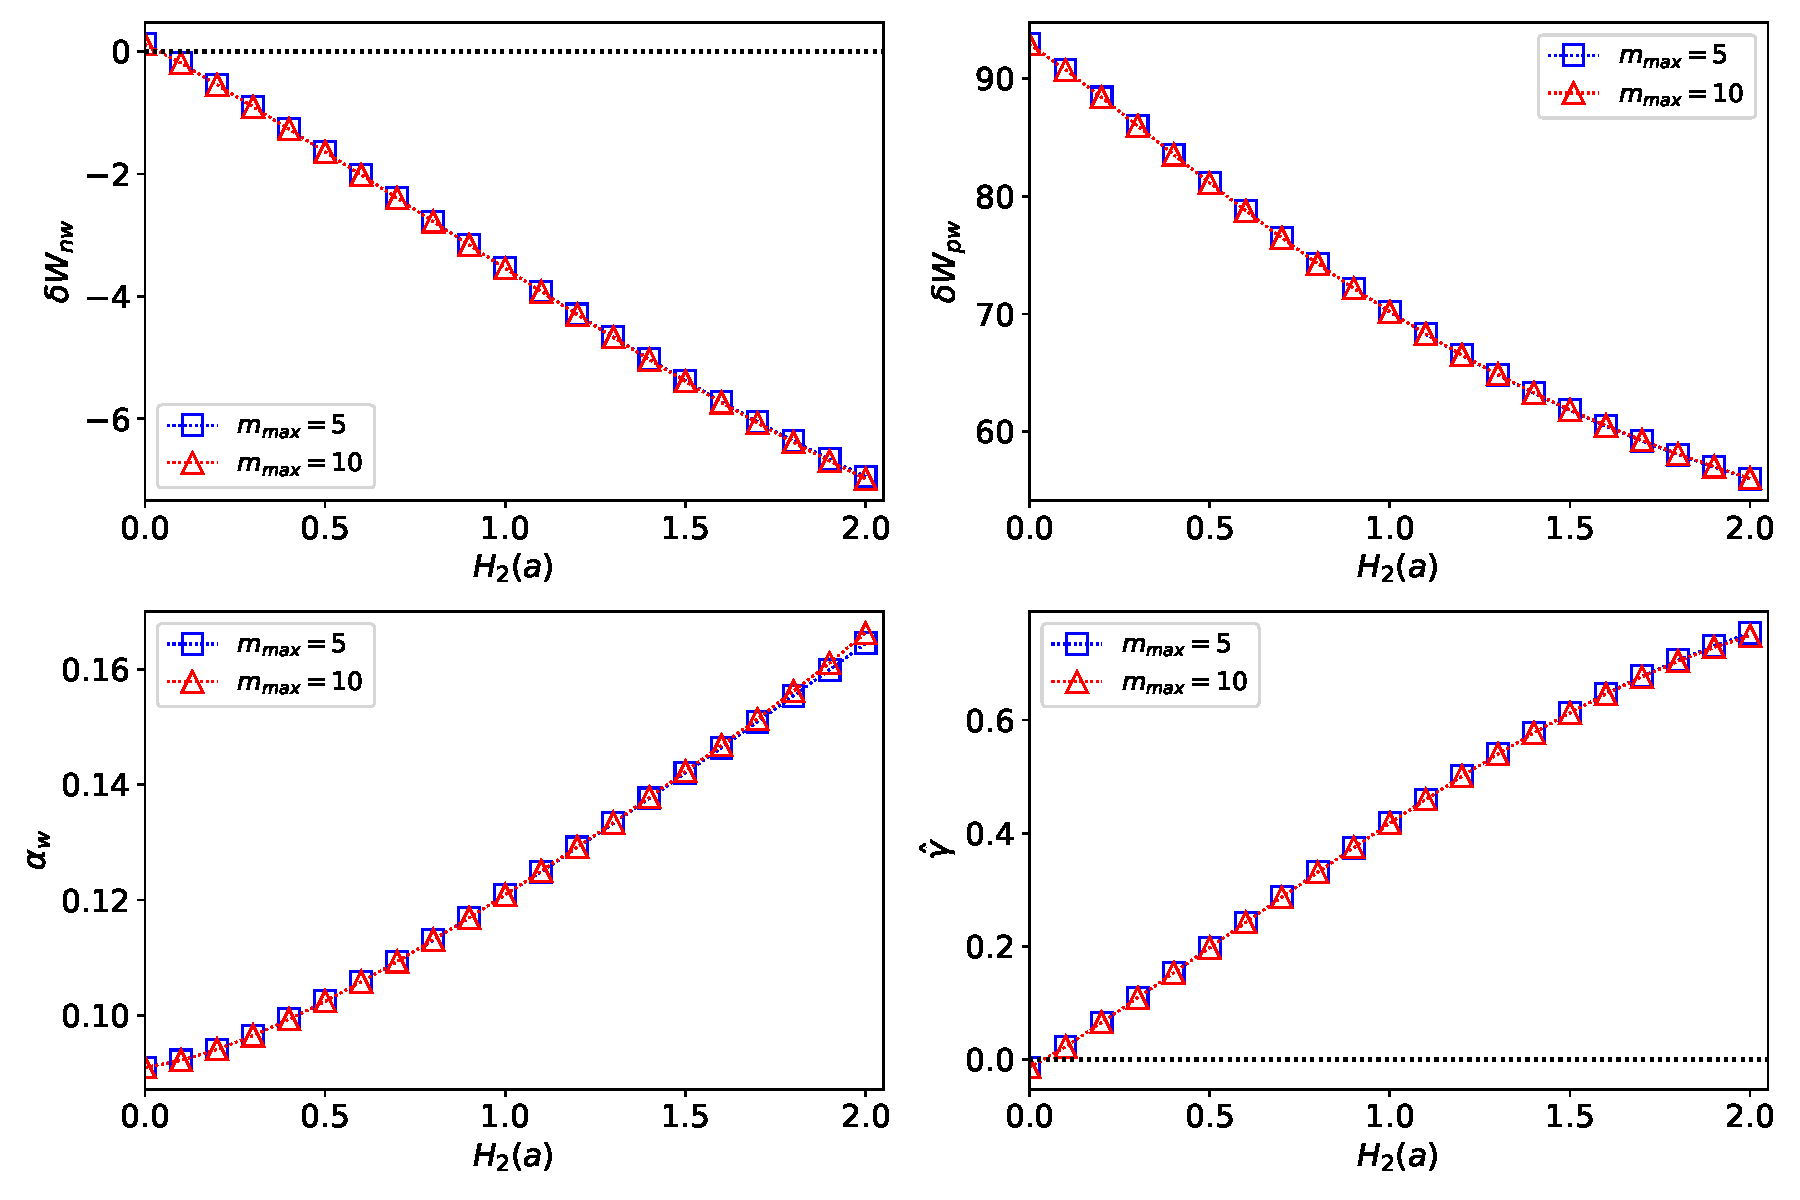
\includegraphics[width=\textwidth]{Fig1.pdf}}
\caption{The no-wall perturbed potential energy, $\delta W_{nw}$, the perfect-wall perturbed potential energy, $\delta W_{pw}$, the wall
parameter, $\alpha_w$, and the normalized thin-wall growth-rate, $\hat{\gamma}$,  of the  vertical mode, plotted as  functions of the
plasma elongation parameter, $H_2(a)$, for plasma equilibria characterized by  $\epsilon=0.1$, $H_3(a)=0$, $q(0)=1.01$, $q(a)=3.6$,  $p_2(0)=0.05$, $\mu=2.5$, and $b_w=1.1$. \label{fig1}}
\end{figure}

\newpage
\begin{figure}
\centerline{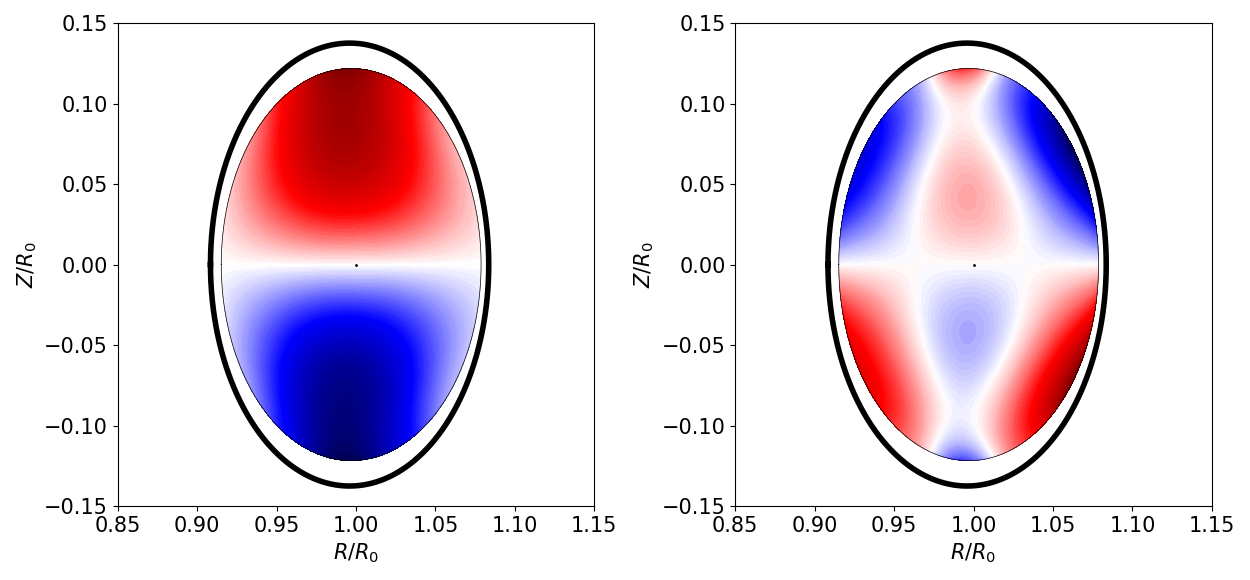
\includegraphics[width=\textwidth]{Fig2.png}}
\caption{The radial plasma displacement function, $y(r,\theta)=f\,\xi^{\,r}$ (left panel), and the perturbed poloidal magnetic
field function, ${\cal Z}(r,\theta)= - b_\theta$ (right panel), of the vertical  mode  for the case $H_2(a)=2$ that features in Fig.~\ref{fig1}.
Here, red is positive and blue is negative. The thick black line indicates the wall. \label{fig2}}
\end{figure}

\begin{figure}
\centerline{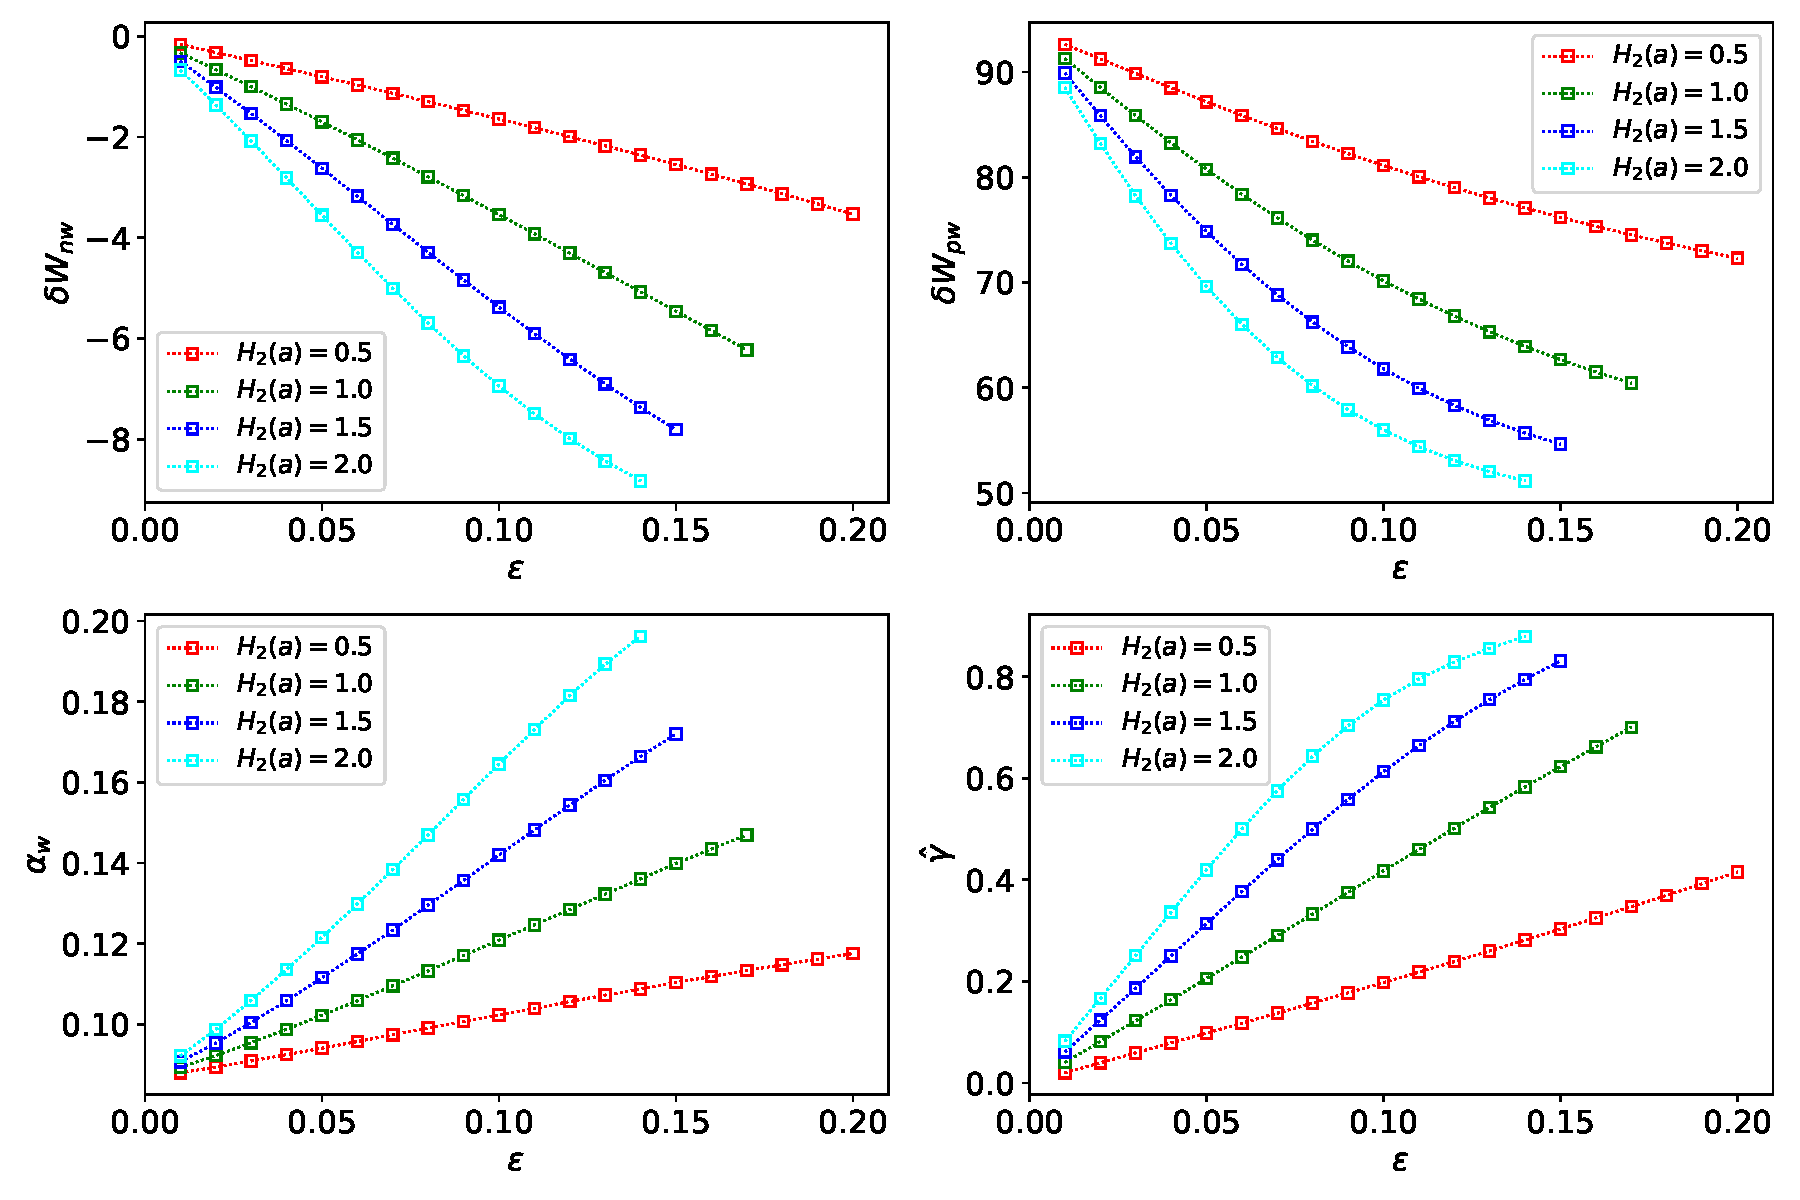
\includegraphics[width=\textwidth]{Fig3.pdf}}
\caption{The no-wall perturbed potential energy, $\delta W_{nw}$, the perfect-wall perturbed potential energy, $\delta W_{pw}$, the wall
parameter, $\alpha_w$, and the normalized thin-wall growth-rate, $\hat{\gamma}$,  of the  vertical mode, plotted as  functions of the
plasma  inverse aspect-ratio, $\epsilon$, for plasma equilibria characterized by   $H_3(a)=0$, $q(0)=1.01$, $q(a)=3.6$,  $p_2(0)=0.05$, $\mu=2.5$, $b_w=1.1$, and
various different values of $H_2(a)$.  \label{fig3}}
\end{figure}

\begin{figure}
\centerline{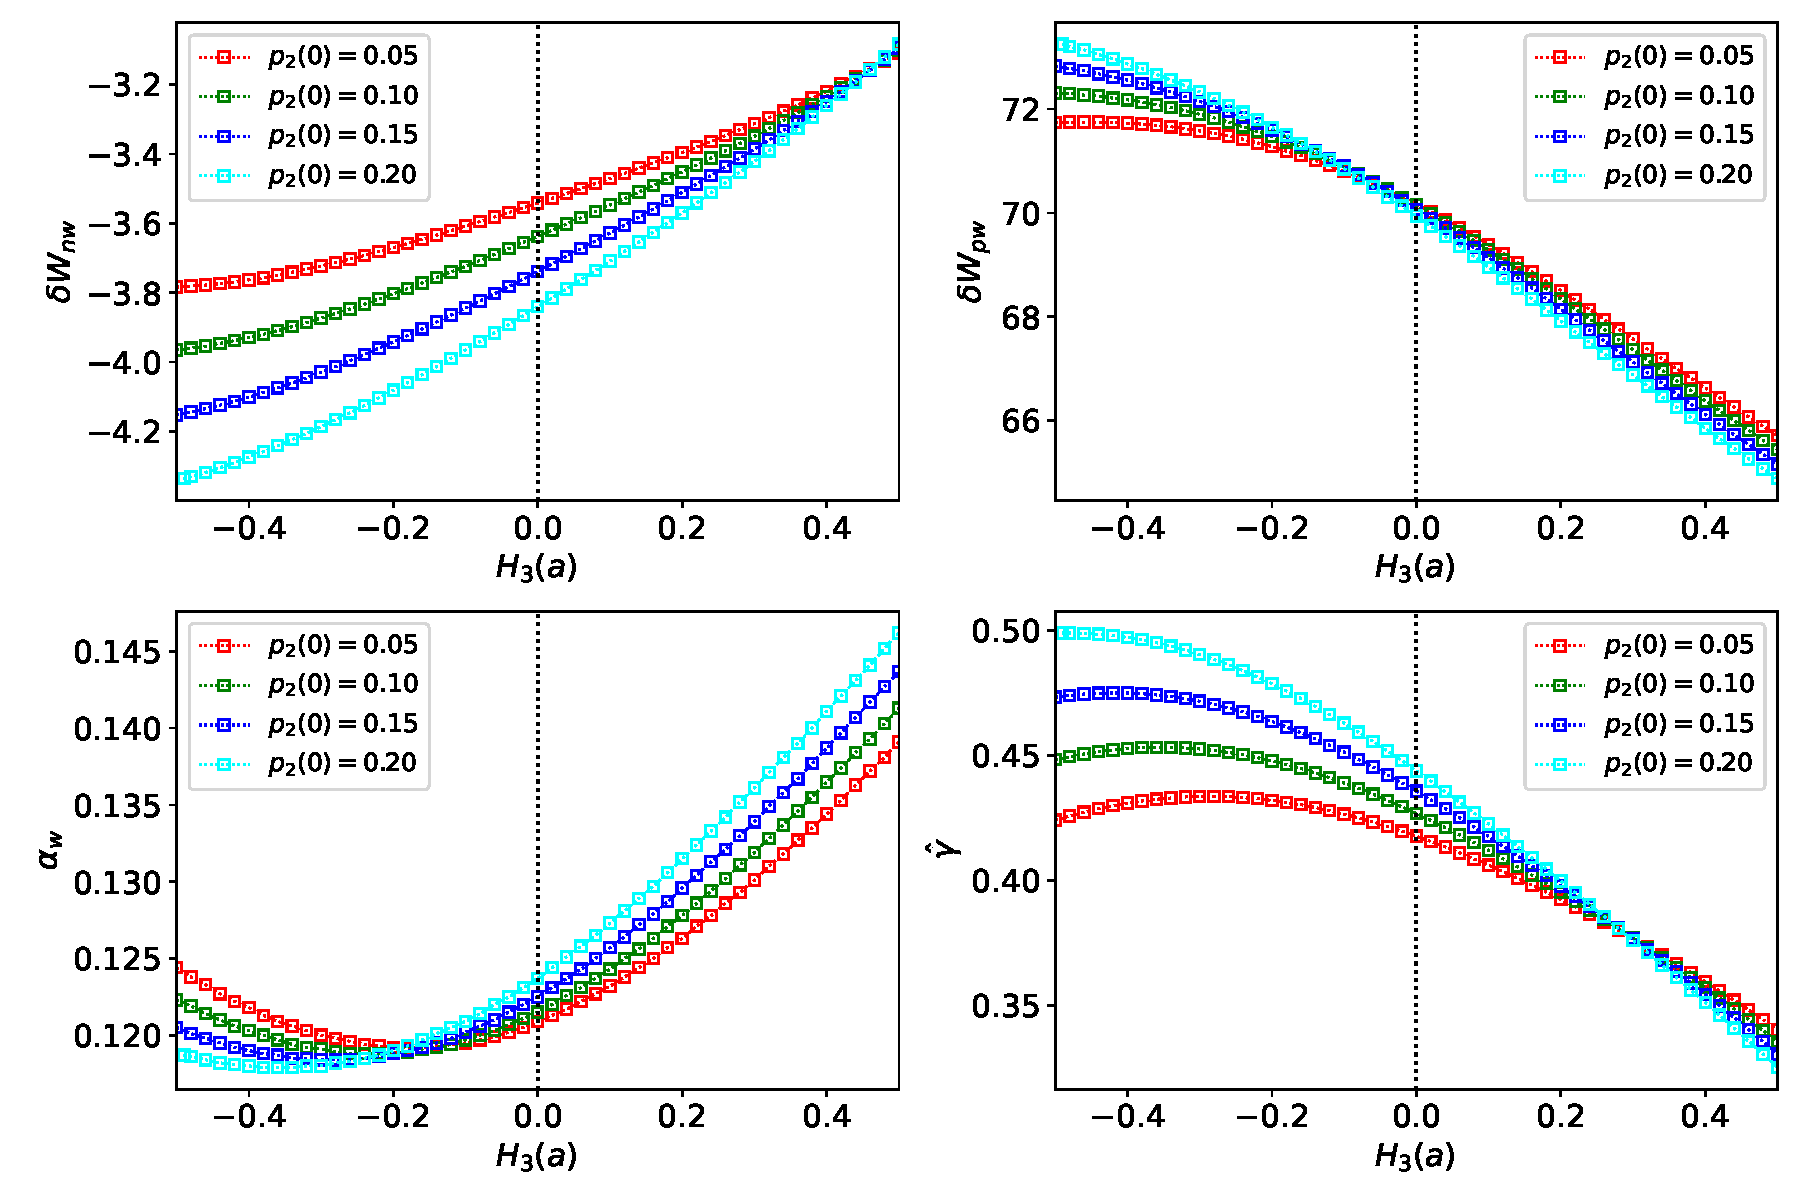
\includegraphics[width=\textwidth]{Fig4.pdf}}
\caption{The no-wall perturbed potential energy, $\delta W_{nw}$, the perfect-wall perturbed potential energy, $\delta W_{pw}$, the wall
parameter, $\alpha_w$, and the normalized thin-wall growth-rate, $\hat{\gamma}$,  of the  vertical  mode, plotted as  functions of the
plasma triangularity parameter, $H_3(a)$, for plasma equilibria characterized by  $\epsilon=0.1$, $H_2(a)=1$, $q(0)=1.01$, $q(a)=3.6$,  $\mu=2.5$, $b_w=1.1$, and
various different values of $p_2(0)$.  \label{fig4}}
\end{figure}

\newpage
\begin{figure}
\centerline{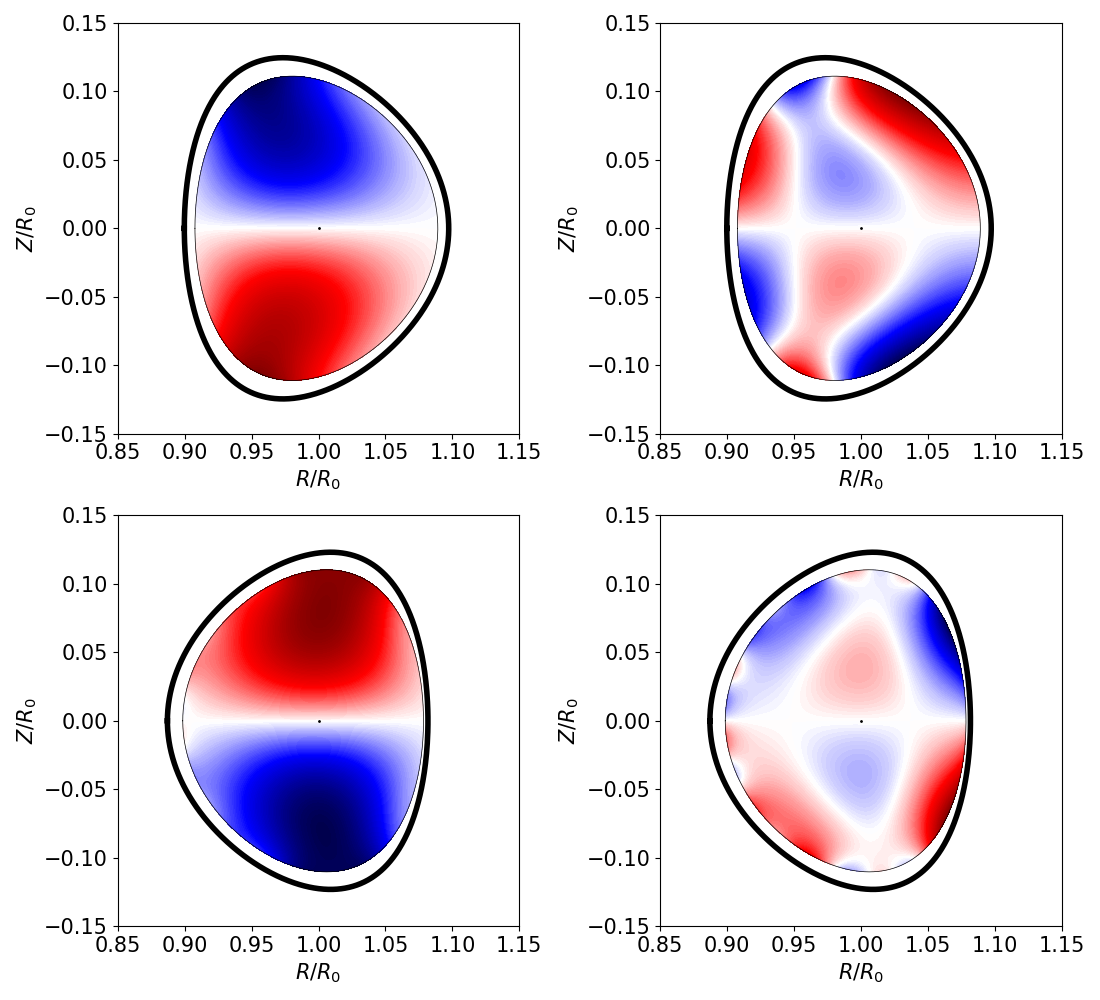
\includegraphics[width=\textwidth]{Fig5.png}}
\caption{The radial plasma displacement function, $y(r,\theta)=f\,\xi^{\,r}$ (left panels),  and the perturbed poloidal magnetic
field function, ${\cal Z}(r,\theta)= - b_\theta$ (right panels), of the vertical mode for the cases $H_3(a)=+0.5$, $p_2(0)=0.2$ (top panels) and $H_3(a)=-0.5$, $p_2(0)=0.2$  (bottom panels) that feature in Fig.~\ref{fig4}.
Here, red is positive and blue is negative. The thick black line indicates the wall. \label{fig5}}
\end{figure}

\newpage
\begin{figure}
\centerline{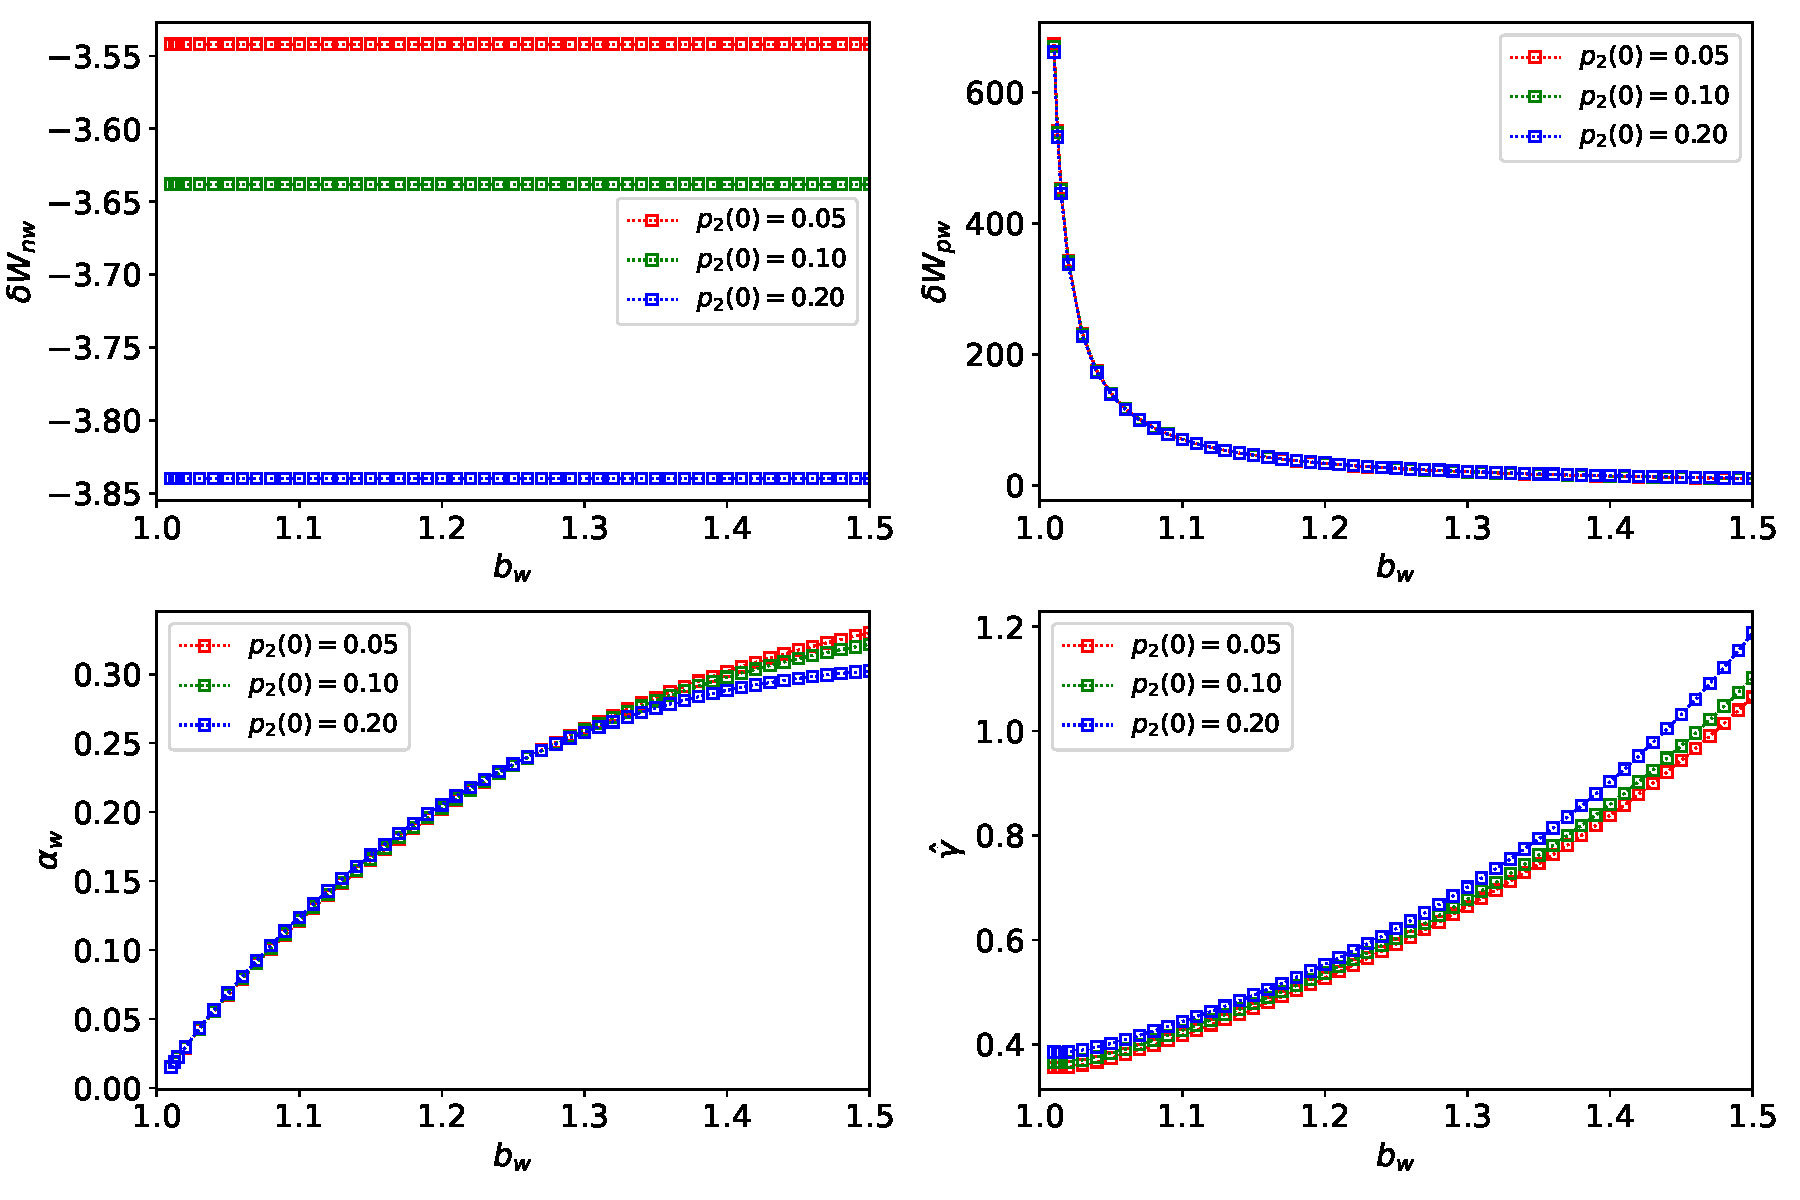
\includegraphics[width=\textwidth]{Fig6.pdf}}
\caption{The no-wall perturbed potential energy, $\delta W_{nw}$, the perfect-wall perturbed potential energy, $\delta W_{pw}$, the wall
parameter, $\alpha_w$, and the normalized thin-wall growth-rate, $\hat{\gamma}$,  of thevertical mode, plotted as  functions of the
relative wall radius, $b_w$, for plasma equilibria characterized by  $\epsilon=0.1$, $H_2(a)=1$, $H_3(a)=0$, $q(0)=1.01$, $q(a)=3.6$, $\mu=2.5$, and various different values of $p_2(0)$.\label{fig6}}
\end{figure}

\newpage
\begin{figure}
\centerline{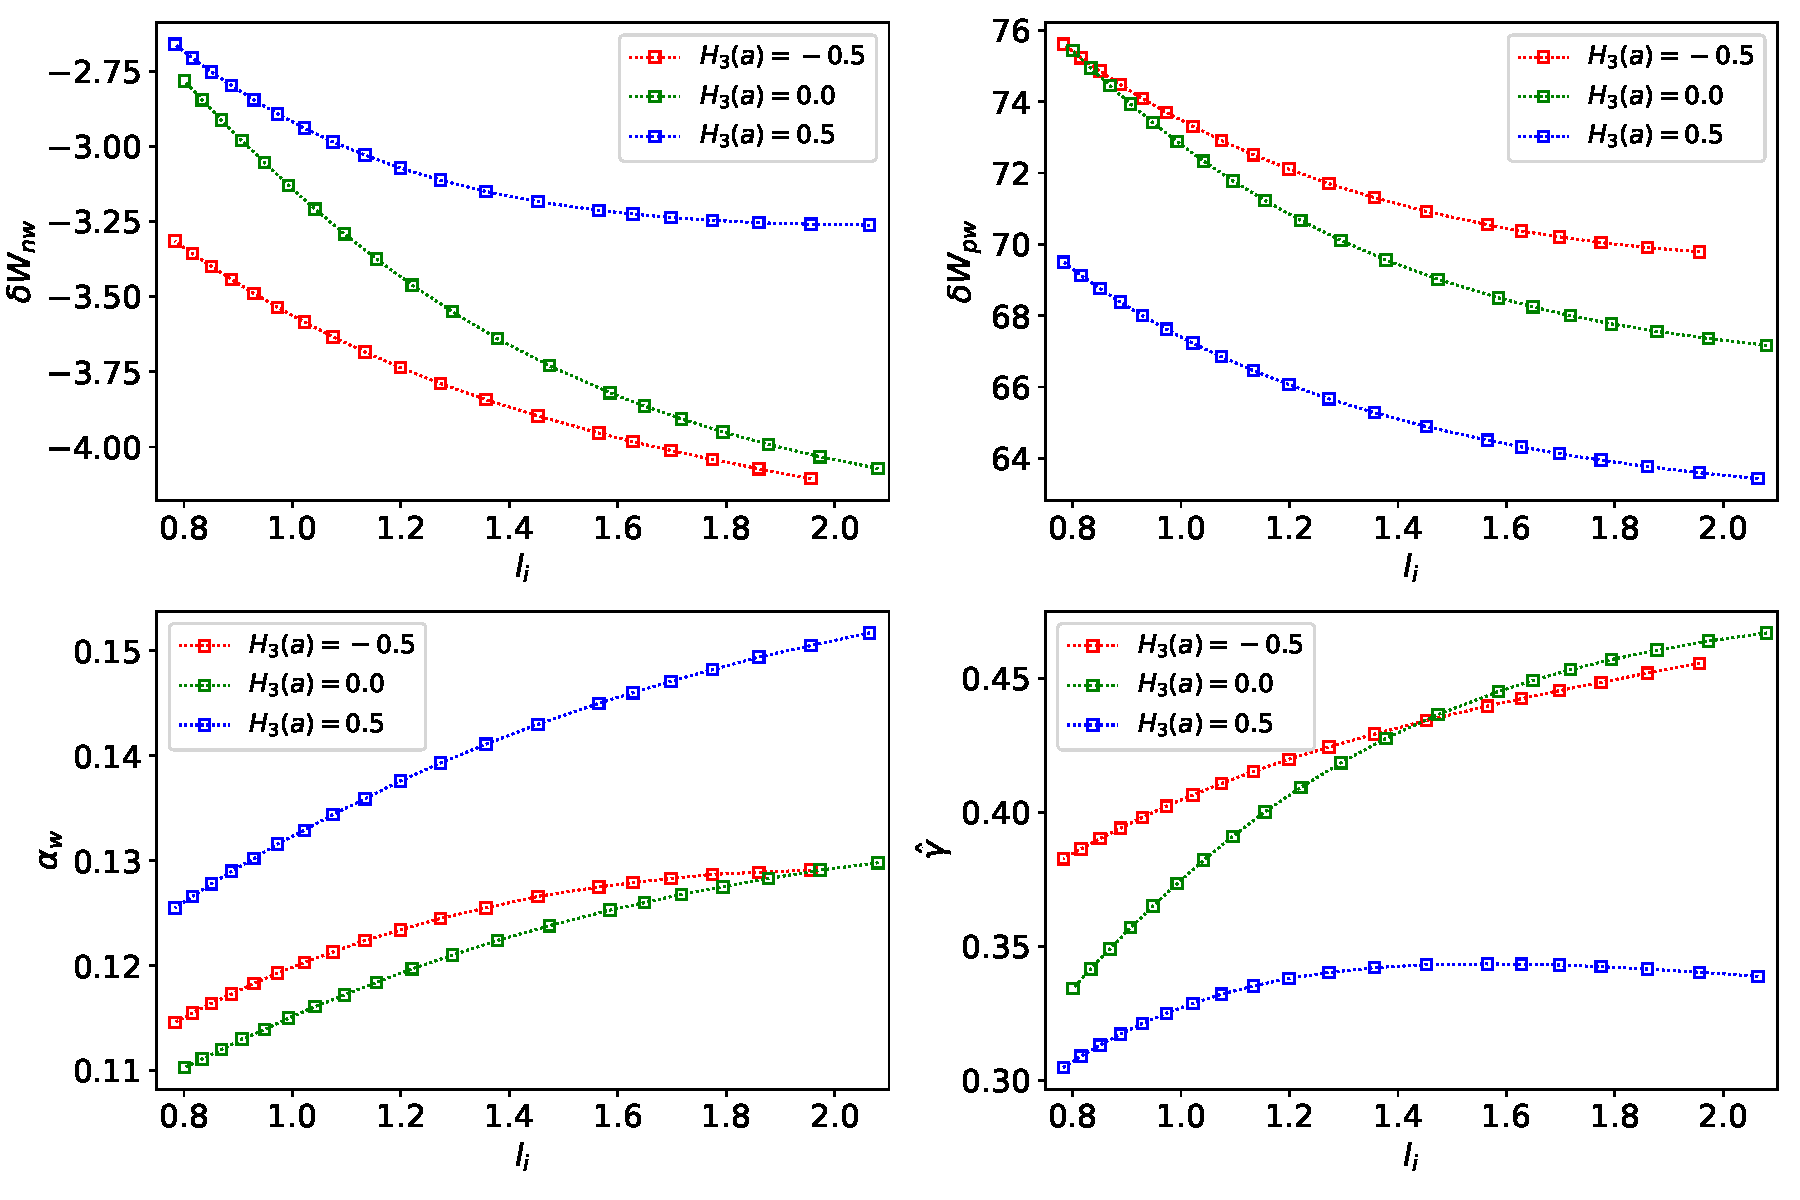
\includegraphics[width=\textwidth]{Fig7.pdf}}
\caption{The no-wall perturbed potential energy, $\delta W_{nw}$, the perfect-wall perturbed potential energy, $\delta W_{pw}$, the wall
parameter, $\alpha_w$, and the normalized thin-wall growth-rate, $\hat{\gamma}$,  of the vertical mode, plotted as  functions of the
plasma self-inductance, $l_i$, for plasma equilibria characterized by  $\epsilon=0.1$, $H_2(a)=1$,   $q(a)=3.6$, $p_2=0.05$, $\mu=2.5$, and various different values of $H_3(a)$.\label{fig7}}
\end{figure}

\newpage
\begin{figure}
\centerline{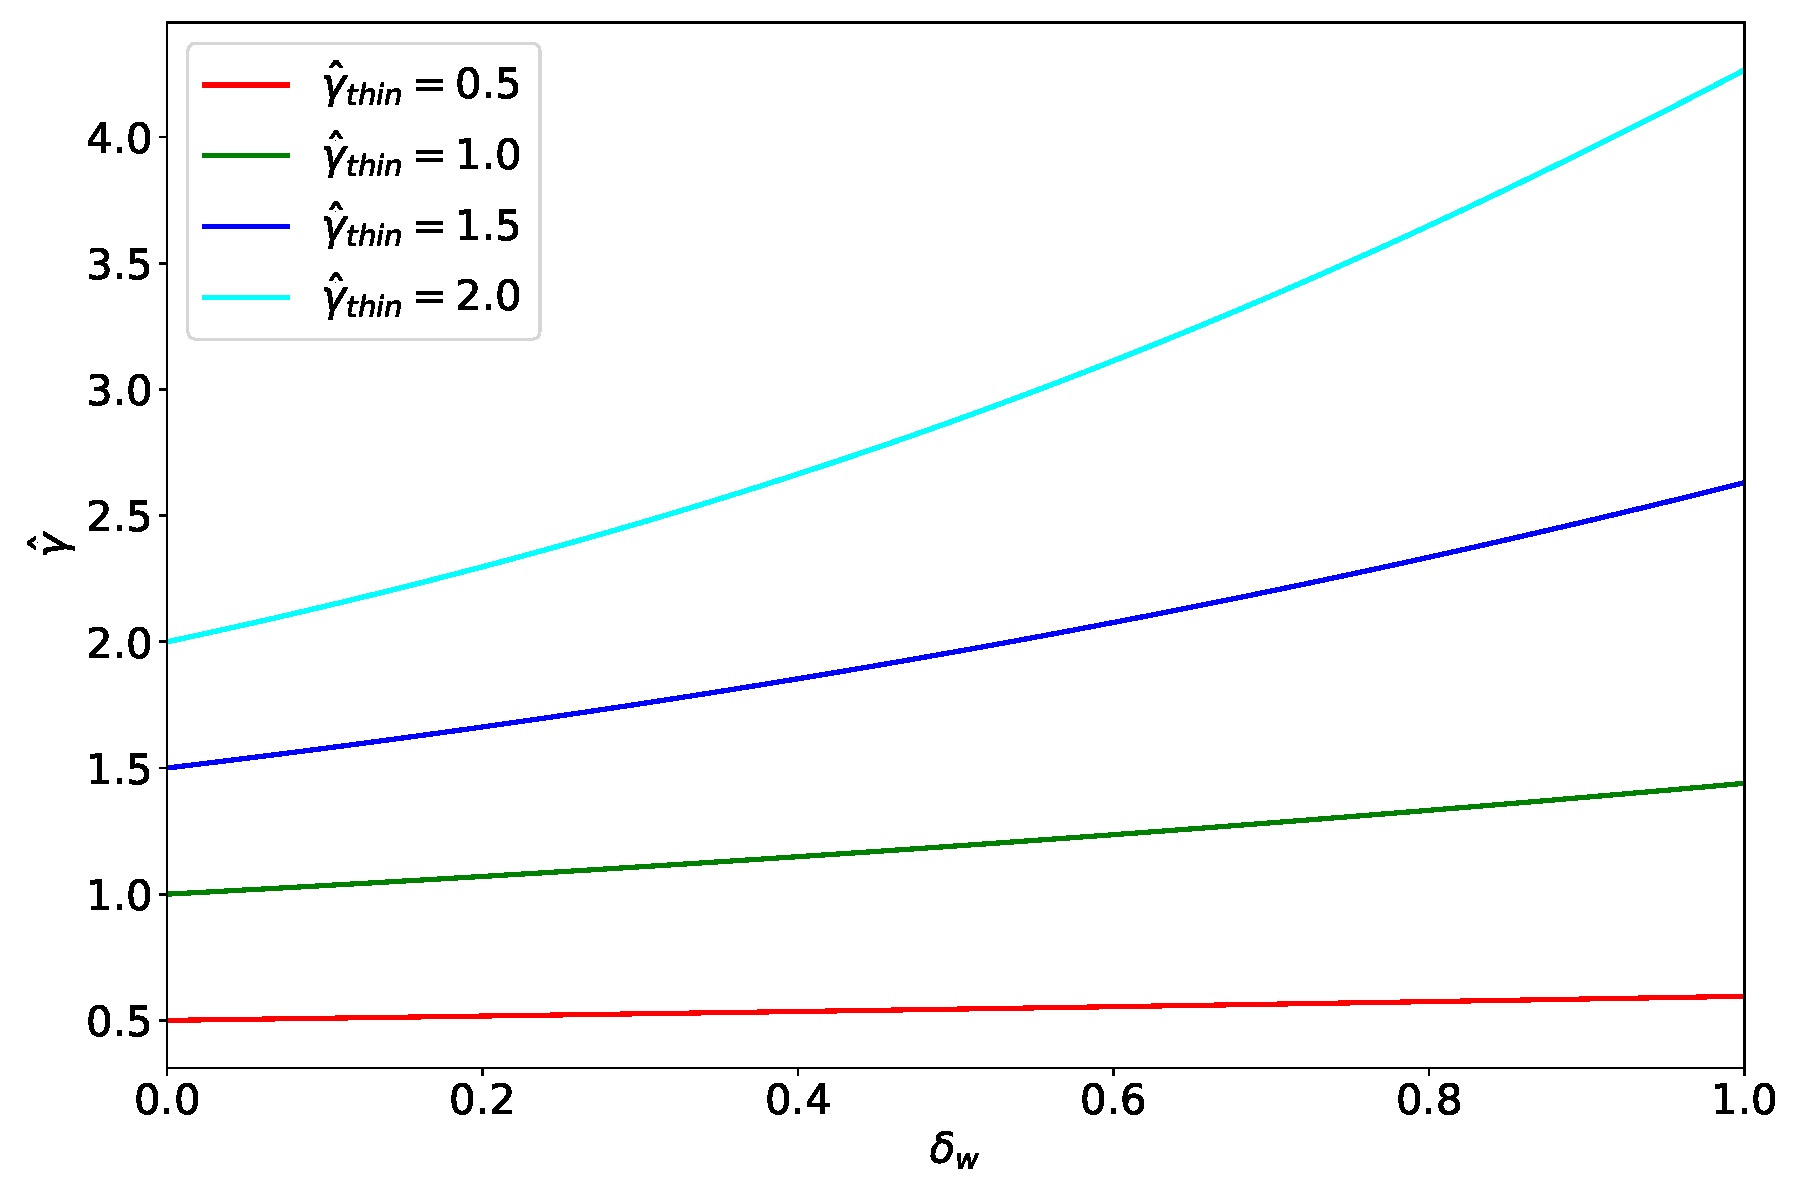
\includegraphics[width=\textwidth]{Fig8.pdf}}
\caption{Variation of the true  normalized resistive wall  mode growth-rate, $\hat{\gamma}$,  with the wall thickness parameter, $\delta_w$, for various values of the thin-wall normalized growth-rate, $\hat{\gamma}_{\rm thin}$.  \label{fig10}}
\end{figure}

\end{document}